% !Mode:: "TeX:UTF-8"
\chapter{后端1}
\begin{mdframed}  
	\textbf{主要目标}
	\begin{enumerate}[labelindent=0em,leftmargin=1.5em]
		\item 理解后端的概念。
		\item 理解以EKF为代表的滤波器后端工作原理。
		\item 理解非线性优化的后端,明白稀疏性是如何利用的。
		\item 使用g2o和Ceres实际操作后端优化。
	\end{enumerate}
\end{mdframed}

本讲开始,我们转入SLAM系统的另一个重要模块:后端优化。

我们看到,前端视觉里程计能给出一个短时间内的轨迹和地图,但由于不可避免的误差累积,这个地图在长时间内是不准确的。所以,在视觉里程计的基础上,我们还希望构建一个尺度、规模更大的优化问题,以考虑长时间内的最优轨迹和地图。不过,考虑到精度与性能的平衡,实际当中存在着许多不同的做法。

\newpage
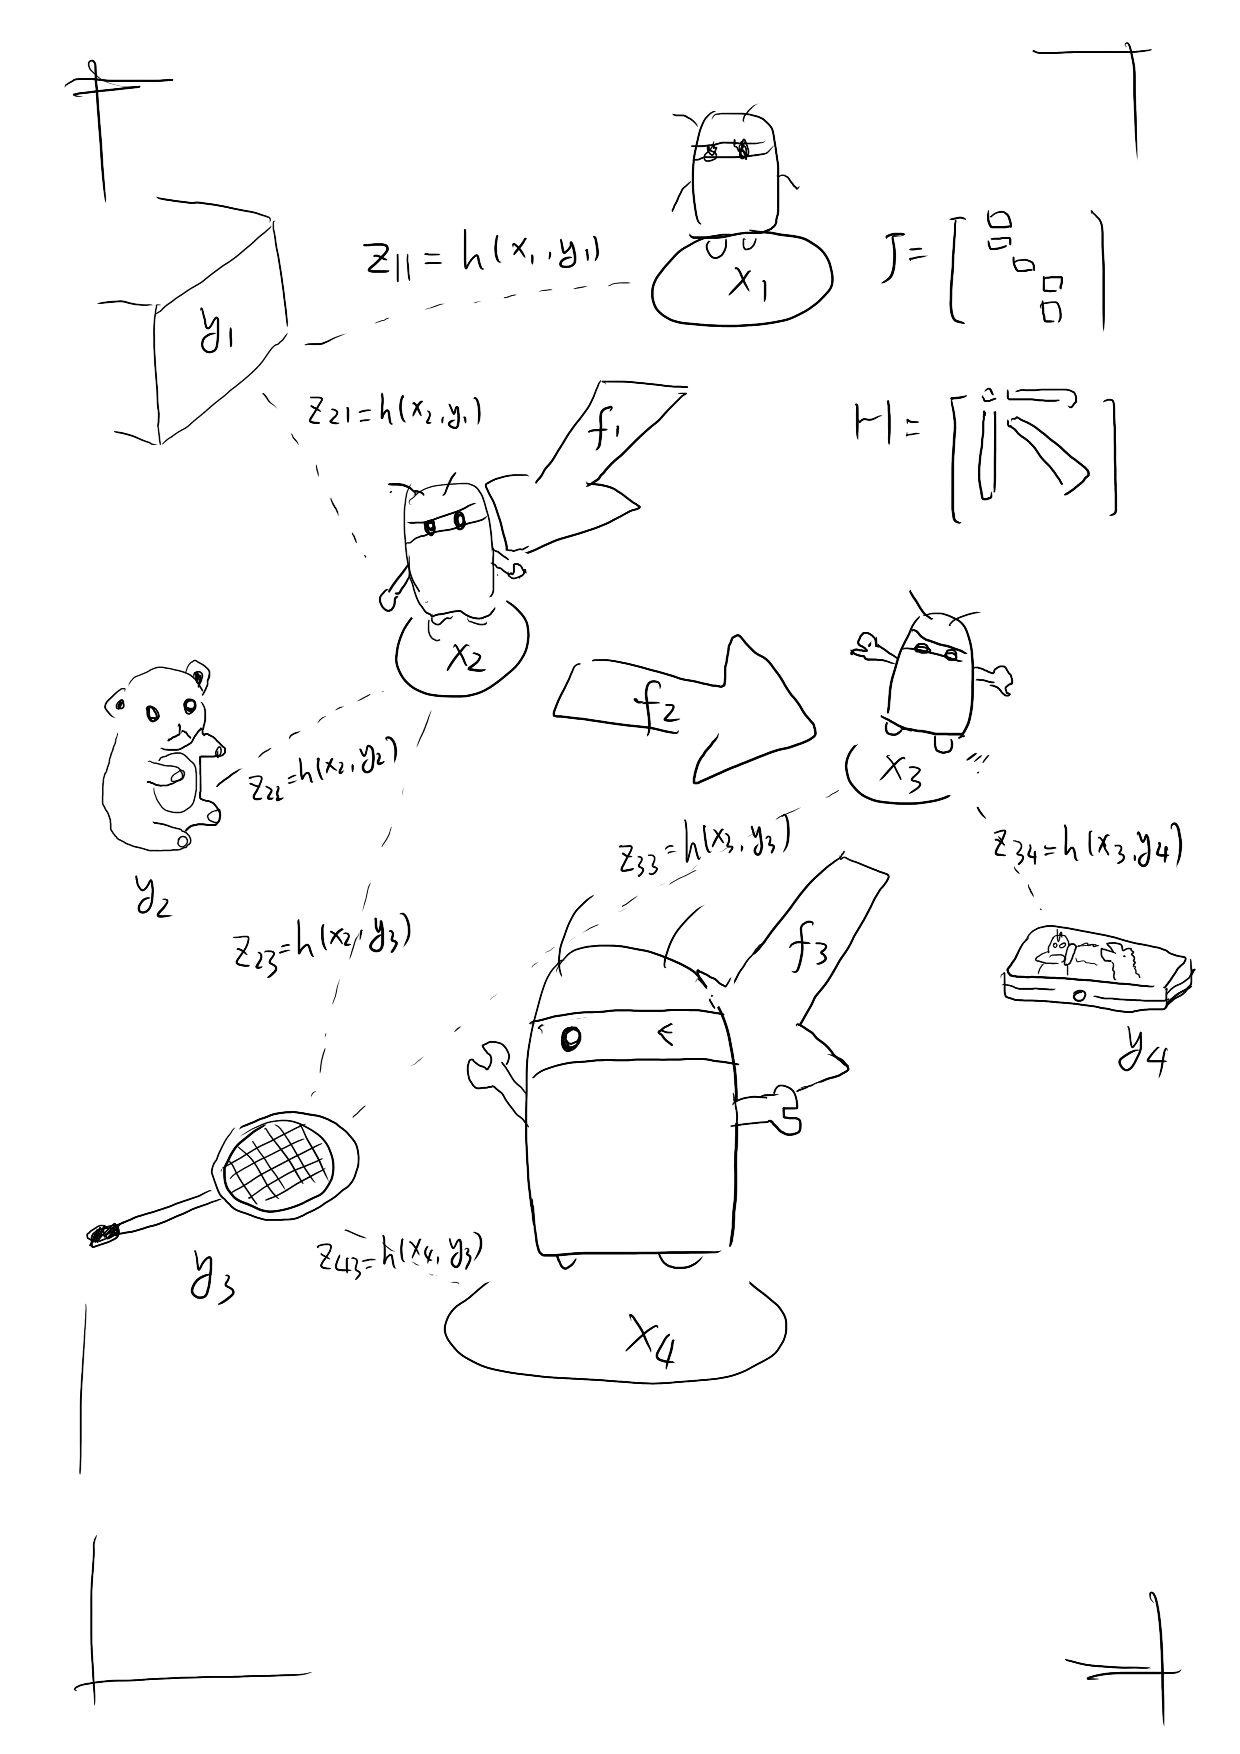
\includepdf{resources/other/ch10.pdf}

\newpage
\section{概述}
\subsection{状态估计的概率解释}
第2讲中提到,视觉里程计只有短暂的记忆,而我们希望整个运动轨迹在较长时间内都能保持最优的状态。我们可能会用最新的知识,更新较久远的状态——站在“久远的状态”的角度上看,仿佛是未来的信息告诉它“你应该在哪里”。所以,在后端优化中,我们通常考虑一段更长时间内(或所有时间内)的状态估计问题,而且不仅使用过去的信息更新自己的状态,也会用未来的信息来更新自己,这种处理方式不妨称为“批量的”(Batch)。否则,如果当前的状态只由过去的时刻决定,甚至只由前一个时刻决定,那不妨称为“渐进的”(Incremental)。

我们已经知道SLAM过程可以由运动方程和观测方程来描述。那么,假设在$t=0$到$t=N$的时间内,有位姿$\bm{x}_0$到$\bm{x}_N$,并且有路标$\bm{y}_1, \cdots, \bm{y}_M$。按照之前的写法,运动和观测方程为
\begin{equation}
\left\{ \begin{array}{l}
{\bm{x}_k} = f\left( {{\bm{x}_{k - 1}},{\bm{u}_k}} \right) + \bm{w}_k \\
{\bm{z}_{k,j}} = h\left( {{ \bm{y}_j},{ \bm{x}_k}}  \right)+ \bm{v}_{k,j}
   \end{array} \right. \quad k=1, \ldots, N, \  j=1, \ldots, M.
\end{equation}

注意以下几点:

\begin{enumerate}
	\item 观测方程中,只有当$\bm{x}_k$看到了$\bm{y}_j$时,才会产生观测数据,否则就没有。事实上,在一个位置通常只能看到一小部分路标。而且,由于视觉SLAM特征点数量众多,所以实际当中观测方程的数量会远远大于运动方程。
	\item 我们可能没有测量运动的装置,所以也可能没有运动方程。在这个情况下,有若干种处理方式:认为确实没有运动方程,或假设相机不动,或假设相机匀速运动。这几种方式都是可行的。在没有运动方程的情况下,整个优化问题就只由许多个观测方程组成。这就非常类似于SfM(Structure from Motion)问题,相当于我们通过一组图像来恢复运动和结构。与SfM中不同的是,SLAM中的图像有时间上的先后顺序,而SfM中允许使用完全无关的图像。
\end{enumerate}

我们知道每个方程都受噪声影响,所以要把这里的位姿$\bm{x}$和路标$\bm{y}$看成\textbf{服从某种概率分布的随机变量},而不是单独的一个数。因此,我们关心的问题就变成:当我拥有某些运动数据$\bm{u}$和观测数据$\bm{z}$时,如何来确定状态量$\bm{x}, \bm{y}$的分布?进而,如果得到了新时刻的数据,那么它们的分布又将发生怎样的变化?在比较常见且合理的情况下,我们假设状态量和噪声项服从高斯分布——这意味着在程序中只需要储存它们的均值和协方差矩阵即可。均值可看作是对变量最优值的估计,而协方差矩阵则度量了它的不确定性。那么,问题就转变为:当存在一些运动数据和观测数据时,我们如何去估计状态量的高斯分布?

我们依然设身处地地扮演一下小萝卜。只有运动方程时,相当于我们蒙着眼睛在一个未知的地方走路。尽管我们知道自己每一步走了多远,但是随着时间增长,我们将对自己的位置越来越不确定——内心也就越不安。这说明在输入数据受噪声影响时,我们对位置方差的估计将越来越大。但是,当我们睁开眼睛时,由于能够不断地观测到外部场景,使得位置估计的不确定性变小,我们就会越来越自信。如果用椭圆或椭球直观地表达协方差阵,那么这个过程有点像是在手机地图软件中走路的感觉。以\autoref{fig:uncertainty}~为例,读者可以想象,当没有观测数据时,这个圆会随着运动越来越大;而如果有正确的观测,圆就会缩小至一定的大小,保持稳定。

\begin{figure}[!ht]
	\centering
	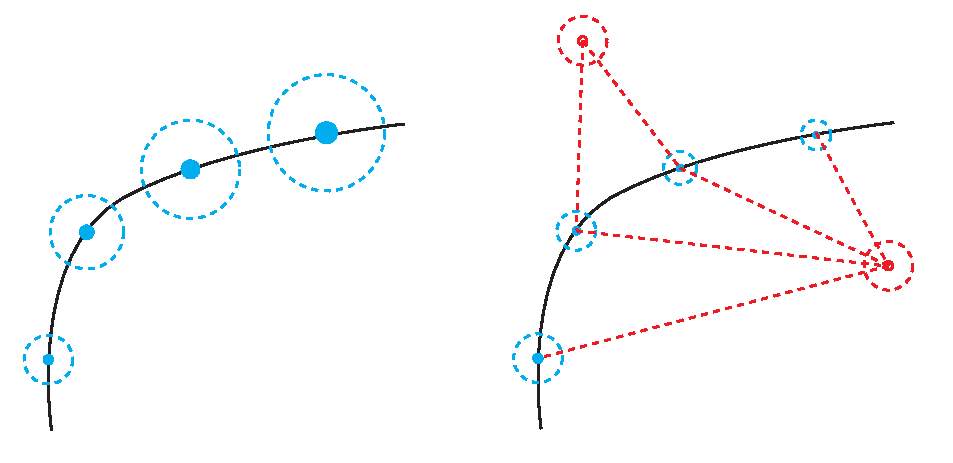
\includegraphics[width=0.66\textwidth]{backend1/uncertainty.pdf}
	\caption{不确定性的直观描述。左侧:只有运动方程时,由于下一时刻的位姿是在上一时刻基础上添加了噪声,所以不确定性越来越大。右侧:存在路标点时,不确定性会明显减小。不过请注意,这只是一个直观的示意图,并非实际数据。}
	\label{fig:uncertainty}
\end{figure}

上面的过程以比喻的形式解释了状态估计中的问题,下面我们要以定量的方式来看待它。在第6讲中,我们介绍了最大似然估计,提到把状态估计转换为最小二乘的做法。在本讲我们要更仔细地讨论这个问题。首先,由于位姿和路标点都是待估计的变量,我们改变一下记号,令$\bm{x}_k$为$k$时刻的所有未知量。它包含了当前时刻的相机位姿与$m$个路标点。在这种记号的意义下(虽然与之前稍有不同,但含义是清楚的),写成:
\begin{equation}
\bm{x}_k  \buildrel \Delta \over =  \{ \bm{x}_k, \bm{y}_1, \ldots, \bm{y}_m \}.
\end{equation}

同时,把$k$时刻的所有观测记作$\bm{z}_k$。于是,运动方程与观测方程的形式可写得更加简洁。这里不会出现$\bm{y}$,但我们心里要明白这时$\bm{x}$中已经包含了之前的$\bm{y}$:
\begin{equation}
\left\{ \begin{array}{l}
{\bm{x}_k} = f\left( {{\bm{x}_{k - 1}},{\bm{u}_k}} \right) + \bm{w}_k \\
{\bm{z}_{k}} = h\left( \bm{x}_k  \right)+ \bm{v}_{k}
\end{array} \right. \quad k=1, \ldots, N .
\end{equation}

现在考虑第$k$时刻的情况。我们希望用过去$0$到$k$中的数据来估计现在的状态分布:
\begin{equation}
P(\bm{x}_k | \bm{x}_0, \bm{u}_{1:k}, \bm{z}_{1:k}).
\end{equation}

下标$0:k$表示从$0$时刻到$k$时刻的所有数据。请注意,$\bm{z}_k$表示所有在$k$时刻的观测数据,它可能不止一个,只是这种记法更加方便。

下面我们来看如何对状态进行估计。按照贝叶斯法则,把$\bm{z}_k$与$\bm{x}_k$交换位置,有:
\begin{equation}
\label{eq:10-5}
P\left( {{\bm{x}_k}|{\bm{x}_0},{\bm{u}_{1:k}},{\bm{z}_{1:k}}} \right) \propto P\left( {{\bm{z}_k}|{\bm{x}_k}} \right) P\left( {{\bm{x}_k}|{\bm{x}_0},{\bm{u}_{1:k}},{\bm{z}_{1:k - 1}}} \right).
\end{equation}

读者应该不会感到陌生。这里第一项称为\textbf{似然},第二项称为\textbf{先验}。似然由观测方程给定,而先验部分,我们要明白当前状态$\bm{x}_k$是基于过去所有的状态估计得来的。至少,它会受$\bm{x}_{k-1}$影响,于是按照$\bm{x}_{k-1}$时刻为条件概率展开:
\begin{equation}
\label{eq:bayes-estimator}
P\left( {{\bm{x}_k}|{\bm{x}_0},{\bm{u}_{1:k}},{\bm{z}_{1:k - 1}}} \right) = \int {P\left( {{\bm{x}_k}|{\bm{x}_{k - 1}},{\bm{x}_0},{\bm{u}_{1:k}},{\bm{z}_{1:k - 1}}} \right)P\left( {{\bm{x}_{k - 1}}|{\bm{x}_0},{\bm{u}_{1:k}},{\bm{z}_{1:k - 1}}} \right) \mathrm{d}\bm{x}_{k-1} }.
\end{equation}

如果考虑更久之前的状态,也可以继续对此式进行展开,但现在我们只关心$k$时刻和$k-1$时刻的情况。至此,我们给出了贝叶斯估计,虽然上式还没有具体的概率分布形式,所以还没法实际地操作它。对这一步的后续处理,方法上产生了一些分歧。大体上讲,存在若干种选择:其一是假设\textbf{马尔可夫性},简单的一阶马氏性认为,$k$时刻状态只与$k-1$时刻状态有关,而与再之前的无关。如果做出这样的假设,我们就会得到以\textbf{扩展卡尔曼滤波}(EKF)为代表的滤波器方法。在滤波方法中,我们会从某时刻的状态估计,推导到下一个时刻。另外一种方法是依然考虑$k$时刻状态与之前\textbf{所有}状态的关系,此时将得到\textbf{非线性优化}为主体的优化框架。非线性优化的基本知识已在前文介绍过。目前视觉SLAM的主流为非线性优化方法。不过,为了让本书更全面,我们要先介绍一下卡尔曼滤波器和EKF的原理。

\subsection{线性系统和KF}
我们首先来看滤波器模型。当我们假设了马尔可夫性,从数学角度会发生哪些变化呢?首先,当前时刻状态只和上一个时刻有关,式\eqref{eq:bayes-estimator}中右侧第一部分可进一步简化:
\begin{equation}
P\left( {{\bm{x}_k}|{\bm{x}_{k - 1}},{\bm{x}_0},{\bm{u}_{1:k}},{\bm{z}_{1:k - 1}}} \right) = P\left( {{\bm{x}_k}|{\bm{x}_{k - 1}},{\bm{u}_k}} \right).
\end{equation}

这里,由于$k$时刻状态与$k-1$之前的无关,所以就简化成只与$\bm{x}_{k-1}$和$\bm{u}_k$有关的形式,与${k}$时刻的运动方程对应。第二部分可简化为
\begin{equation}
P\left( {{\bm{x}_{k - 1}}|{\bm{x}_0},{\bm{u}_{1:k}},{\bm{z}_{1:k - 1}}} \right) = P\left( {{\bm{x}_{k - 1}}|{\bm{x}_0},{\bm{u}_{1:k - 1}},{\bm{z}_{1:k - 1}}} \right).
\end{equation}

这是考虑到$k$时刻的输入量$\bm{u}_k$与$k-1$时刻的状态无关,所以我们把$\bm{u}_k$拿掉。可以看到,这一项实际上是$k-1$时刻的状态分布。于是,这一系列方程说明,我们实际在做的是“如何把$k-1$时刻的状态分布推导至$k$时刻”这样一件事。也就是说,在程序运行期间,我们只要维护一个状态量,对它不断地进行迭代和更新即可。进一步,如果假设状态量服从高斯分布,那么我们只需考虑维护状态量的均值和协方差即可。

我们从形式最简单的线性高斯系统开始,最后会得到卡尔曼滤波器。线性高斯系统是说,运动方程和观测方程可以由线性方程来描述:
\begin{equation}
\left\{ \begin{array}{l}
{\bm{x}_k} = \bm{A}_k {{\bm{x}_{k - 1}}+{\bm{u}_k}} + \bm{w}_k \\
{\bm{z}_{k}} = \bm{C}_k  { \bm{x}_k} + \bm{v}_{k} \end{array} \right. \quad k=1, \ldots, N .
\end{equation}
并假设所有的状态和噪声均满足高斯分布。记这里的噪声服从零均值高斯分布:
\begin{equation}
\bm{w}_k \sim N(\bm{0}, \bm{R}). \quad \bm{v}_k \sim N( \bm{0}, \bm{Q}).
\end{equation}

为了简洁,笔者省略了$\bm{R}$和$\bm{Q}$的下标。现在,利用马尔可夫性,假设我们知道了$k-1$时刻的后验(在$k-1$时刻看来)状态估计$\bm{\hat{x}}_{k-1}$及其协方差$\bm{\hat{P}}_{k-1}$,现在要根据$k$时刻的输入和观测数据,确定$\bm{x}_k$的后验分布。为区分推导中的先验和后验,我们在记号上做一点区别:以尖帽子$\bm{\hat{x}}_k$表示后验,以横线$\bar{\bm{x}}$表示先验分布,请读者不要混淆。

卡尔曼滤波器的第一步,通过运动方程确定$\bm{x}_k$的先验分布。根据高斯分布的性质,显然有:
\begin{equation}
P\left( {{\bm{x}_k}|{\bm{x}_0},{\bm{u}_{1:k}},{\bm{z}_{1:k - 1}}} \right) = N\left( {\bm{A}_k {{\hat{\bm{x}}}_{k - 1}} + {\bm{u}_k}, \bm{A}_k\hat{\bm{P}}_{k-1} {\bm{A}_k^\mathrm{T}} + \bm{R}} \right).
\end{equation}

这一步称为\textbf{预测},原理见附录\ref{sec:gauss-example}。它显示了如何从上一个时刻的状态,根据输入信息(但是有噪声)推断当前时刻的状态分布。这个分布也就是先验。记:
\begin{equation}
\bar{\bm{x}}_k = {\bm{A}_k {{\hat{\bm{x}}}_{k - 1}} + {\bm{u}_k}}, \quad \bar{\bm{P}}_k = {\bm{A}_k \hat{\bm{P}}_{k-1} { \bm{A}^\mathrm{T}_k} + \bm{R}}.
\end{equation}

这非常自然。另一方面,由观测方程,我们可以计算在某个状态下应该产生怎样的观测数据:
\begin{equation}
P\left( {{\bm{z}_k}|{\bm{x}_k}} \right) = N\left( {{\bm{C}_k}{\bm{x}_k},\bm{Q}} \right) .
\end{equation}

为了得到后验概率,我们想要计算它们的乘积,也就是由式\eqref{eq:10-5}给出的贝叶斯公式。然而,虽然我们知道最后会得到一个关于$\bm{x}_k$的高斯分布,但计算上是有一点点麻烦的,我们先把结果设为$\bm{x}_k \sim N(\bm{\hat{x}}_k, \bm{\hat{P}}_k )$,那么:
\begin{equation}
N(\bm{\hat{x}}_k, \bm{\hat{P}}_k ) = N\left( {{\bm{C}_k}{\bm{x}_k},\bm{Q}} \right) \cdot N( \bm{\bar{x}}_k, \bm{\bar{P}}_k). 
\end{equation}

这里我们稍微用点讨巧的方法。既然我们已经知道等式两侧都是高斯分布,那就只需比较指数部分即可,而无须理会高斯分布前面的因子部分。指数部分很像是一个二次型的配方,我们来推导一下。首先把指数部分展开,有\footnote{这里的等号并不严格,实际允许相差与$\bm{x}_k$无关的常数。}:
\begin{equation}
{\left( {{\bm{x}_k} - {{\hat{\bm{x}}}_k}} \right)^\mathrm{T}}\hat{\bm{P}}_k^{ - 1}\left( {{\bm{x}_k} - {{\hat{\bm{x}}}_k}} \right) = {\left( {{\bm{z}_k} - {\bm{C}_k} {\bm{x}_k}} \right)^\mathrm{T}}{\bm{Q}^{ - 1}}\left( {{\bm{z}_k} - {\bm{C}_k}{\bm{x}_k}} \right) + {\left( {{\bm{x}_k} - {{\bar{\bm{x}}}_k}} \right)^\mathrm{T}}\bar{\bm{P}}_k^{ - 1}\left( {\bm{x}_k - {{\bar{\bm{x}}}_k}} \right).
\end{equation}

为了求左侧的$\hat{\bm{x}}_k$和$\bm{\hat{P}}_k$,我们把两边展开,并比较$\bm{x}_k$的二次和一次系数。对于二次系数,有:
\begin{equation}
\label{eq:kalman-cov}
\hat{\bm{P}}_k^{ - 1} = \bm{C}_k^\mathrm{T}{\bm{Q}^{ - 1}}{\bm{C}_k} + \bar {\bm{P}}_k^{ - 1}.
\end{equation}

该式给出了协方差的计算过程。为了便于后面列写式子,定义一个中间变量:
\begin{equation}
\label{eq:kalman-K}
\bm{K} = \bm{\hat{P}}_k \bm{C}_k^\mathrm{T} \bm{Q}^{-1}.
\end{equation}

根据此定义,在式\eqref{eq:kalman-cov}的左右各乘$\bm{\hat{P}}_k$,有:
\begin{equation}
\bm{I} = \bm{\hat{P}}_k \bm{C}_k^\mathrm{T} \bm{Q}^{-1} \bm{C}_k + \bm{\hat{P}}_k \bm{\bar{P}}_k^{-1} = \bm{K} \bm{C}_k + \bm{\hat{P}}_k \bm{\bar{P}}_k^{-1}.
\end{equation}

于是有\footnote{这里看似有一点儿循环定义的意思。我们由$\bm{\hat{P}}_k$定义了$\bm{K}$,又把$\bm{\hat{P}}_k$写成了$\bm{K}$的表达式。然而,实际当中$\bm{K}$可以不依靠$\bm{\hat{P}}_k$算得,参见本讲的习题。}:
\begin{equation}
\bm{\hat{P}}_k = ( \bm{I} - \bm{K} \bm{C}_k ) \bm{\bar{P}}_k.
\end{equation}

然后再比较一次项的系数,有:
\begin{equation}
- 2\hat {\bm{x}}_k^\mathrm{T} \hat{\bm{P}}_k^{ - 1}{\bm{x}_k} =  - 2\bm{z}_k^\mathrm{T} {\bm{Q}^{ - 1}}{\bm{C}_k}{\bm{x}_k} - 2\bm{\bar {x}}_k^\mathrm{T} \bm{\bar {P}}_k^{ - 1}{\bm{x}_k}.
\end{equation}

整理(取系数并转置)得:
\begin{equation}
\hat { \bm{P}}_k^{ - 1}{{\hat{\bm{x}}}_k} = \bm{C}_k^\mathrm{T} {\bm{Q}^{ - 1}}{\bm{z}_k} + \bar{\bm{P}}_k^{ - 1}{{\bm{\bar{x}}}_k}.
\end{equation}

两侧乘以$\bm{\hat{P}}_k$并代入式\eqref{eq:kalman-K},得:
\begin{align}
{{\bm{\hat {x}}}_k} &= {{\hat {\bm{P}}}_k} \bm{C}_k^\mathrm{T} { \bm{Q}^{ - 1}}{\bm{z}_k} + {{\bm{\hat{ P}}}_k}\bar {\bm{P}}_k^{ - 1}{{\bar {\bm{x}}}_k}\\
&= \bm{K} {\bm{z}_k} + \left( {\bm{I} - \bm{K}{\bm{C}_k}} \right){{\bm{\bar {x}}}_k} = {{\bar {\bm{x}}}_k} + \bm{K} \left( {\bm{z}_k - {\bm{C}_k}{\bm{\bar{x}}_k}} \right).
\end{align}

于是我们又得到了后验均值的表达。总而言之,上面的两个步骤可以归纳为“预测”(Predict)和“更新”(Update)两个步骤:

\begin{mdframed}
\begin{enumerate}
	\item 预测:
	\begin{equation}
	\bar{\bm{x}}_k = {\bm{A}_k {{\hat{\bm{x}}}_{k - 1}} + {\bm{u}_k}}, \quad \bar{\bm{P}}_k = {\bm{A}_k \hat{\bm{P}}_{k-1} { \bm{A}^\mathrm{T}_k} + \bm{R}}.
	\end{equation}
	\item 更新:
	先计算$\bm{K}$,它又称为卡尔曼增益。
	\begin{equation}
	\label{eq:kalman-K-another}
	\bm{K} = {{\bar {\bm{P}}}_k} \bm{C}_k^\mathrm{T} {\left( {{\bm{C}_k}{{\bar {\bm{P}}}_k}\bm{C}_k^\mathrm{T} + {\bm{Q}_k}} \right)^{ - 1}}.
	\end{equation}
	然后计算后验概率的分布。
	\begin{equation}
	\begin{array}{l}
	\hat {\bm{x}}_k = {{\bar {\bm{x}}}_k} + \bm{K} \left( {\bm{z}_k - {\bm{C}_k}{\bm{\bar{x}}_k}} \right)\\
	{{\bm{\hat {P}}}_k} = \left( {\bm{I} - \bm{K}{\bm{C}_k}} \right) \bar{\bm{P}}_k.
	\end{array}.
	\end{equation}
\end{enumerate}
\end{mdframed}

至此,我们推导了经典的卡尔曼滤波器的整个过程。事实上,卡尔曼滤波器有若干种推导方式,而我们使用的是从概率角度出发的最大后验概率估计的形式。我们看到,在线性高斯系统中,卡尔曼滤波器构成了该系统中的最大后验概率估计。而且,由于高斯分布经过线性变换后仍服从高斯分布,所以整个过程中我们没有进行任何的近似。可以说,卡尔曼滤波器构成了线性系统的最优无偏估计。

\subsection{非线性系统和EKF}
在理解了卡尔曼滤波之后,我们必须要澄清一点:SLAM中的运动方程和观测方程通常是非线性函数,尤其是视觉SLAM中的相机模型,需要使用相机内参模型及李代数表示的位姿,更不可能是一个线性系统。一个高斯分布,经过非线性变换后,往往不再是高斯分布,所以在非线性系统中,我们必须取一定的近似,将一个非高斯分布近似成高斯分布。

我们希望把卡尔曼滤波器的结果拓展到非线性系统中,称为扩展卡尔曼滤波器(Extended Kalman Filter,EKF)。通常的做法是,在某个点附近考虑运动方程及观测方程的一阶泰勒展开,只保留一阶项,即线性的部分,然后按照线性系统进行推导。令$k-1$时刻的均值与协方差矩阵为$\bm{\hat{x}}_{k-1},\bm{\hat{P}}_{k-1}$。在$k$时刻,我们把运动方程和观测方程在$\bm{\hat{x}}_{k-1},\bm{\hat{P}}_{k-1}$处进行\textbf{线性化}(相当于一阶泰勒展开),有:
\begin{equation}
{\bm{x}_k} \approx f\left( {{{\bm{\hat x}}_{k - 1}},{\bm{u}_k}} \right) + {\left. {\frac{{\partial f}}{{\partial {\bm{x}_{k - 1}}}}} \right|_{{{\bm{\hat x}}_{k - 1}}}}\left( {{\bm{x}_{k - 1}} - {{\bm{\hat x}}_{k - 1}}} \right) + {\bm{w}_k}.
\end{equation}

记这里的偏导数为
\begin{equation}
\bm{F} = \left. {\frac{{\partial f}}{{\partial {\bm{x}_{k - 1}}}}} \right|_{{{\bm{\hat x}}_{k - 1}}}.
\end{equation}

同样,对于观测方程,亦有:
\begin{equation}
{\bm{z}_k} \approx h\left( {{{\bm{\bar x}}_k}} \right) + {\left. {\frac{{\partial h}}{{\partial {\bm{x}_k}}}} \right|_{{{\bm{\bar x}}_k}}}\left( {\bm{x}_k - {{\bm{\bar x}}_k}} \right) + {\bm{n}_k}.
\end{equation}

记这里的偏导数为
\begin{equation}
\bm{H} = \left. {\frac{{\partial h}}{{\partial {\bm{x}_k}}}} \right|_{{{\bm{\bar x}}_k}}.
\end{equation}

那么,在\textbf{预测}步骤中,根据运动方程有:
\begin{equation}
P\left( {{\bm{x}_k}|{\bm{x}_0},{\bm{u}_{1:k}},{\bm{z}_{0:k - 1}}} \right)
 = N(f\left( {{{\bm{\hat x}}_{k - 1}},{\bm{u}_k}} \right), \bm{F}\bm{\hat{P}}_{k-1} \bm{F}^\mathrm{T} + \bm{R}_k).
\end{equation}

这些推导和卡尔曼滤波是十分相似的。为方便表述,记这里的先验和协方差的均值为
\begin{equation}
\bm{\bar {x}}_k = f\left( {{{\bm{\hat x}}_{k - 1}},{\bm{u}_k}} \right), \quad \bm{\bar{P}}_k = \bm{F}\bm{\hat{P}}_{k-1} \bm{F}^\mathrm{T} + \bm{R}_k.
\end{equation}

然后,考虑在观测中我们有:
\begin{equation}
P\left( {{\bm{z}_k}|{\bm{x}_k}} \right) = N( h\left( {{{\bm{\bar x}}_k}} \right) + \bm{H} \left( {\bm{x}_k - {{\bm{\bar x}}_k}} \right), \bm{Q}_k ).
\end{equation}

最后,根据最开始的贝叶斯展开式,可以推导出$\bm{x}_k$的后验概率形式。我们略去中间的推导过程,只介绍其结果。读者可以仿照卡尔曼滤波器的方式,推导EKF的预测与更新方程。简而言之,我们会先定义一个\textbf{卡尔曼增益}$\bm{K}_k$:
\begin{equation}
\bm{K}_k = {\bm{\bar{P}}_{k}}{\bm{H}^\mathrm{T}}{\left( {\bm{H}{\bm{\bar P}_k}{\bm{H}^\mathrm{T}} + {\bm{Q}_k}} \right)^{ - 1}}.
\end{equation}

在卡尔曼增益的基础上,后验概率的形式为
\begin{equation}
{{\bm{\hat x}}_k} = {{\bm{\bar x}}_k} + {\bm{K}_k}\left( {{\bm{z}_k} - h\left( {{\bm{\bar x}_k}} \right)} \right),{\bm{\hat P}_k} = \left( {\bm{I} - {\bm{K}_k}{\bm{H}}} \right) \bm{\bar{P}}_k.
\end{equation}

卡尔曼滤波器给出了在线性化之后状态变量分布的变化过程。在线性系统和高斯噪声下,卡尔曼滤波器给出了无偏最优估计。而在SLAM这种非线性的情况下,它给出了单次线性近似下的最大后验估计(MAP)。

\subsection{EKF的讨论}
EKF以形式简洁、应用广泛著称。当想要在某段时间内估计某个不确定量时,我们首先想到的就是EKF。在早期的SLAM中,EKF占据了很长一段时间的主导地位,研究者们讨论了各种各样的滤波器在SLAM中的应用,如IF(信息滤波器)\textsuperscript{\cite{Sujan2005}}、IKF\textsuperscript{\cite{Janabi-Sharifi2010}}(Iterated KF)、UKF\textsuperscript{\cite{Li2010}}(Unscented KF)和粒子滤波器\textsuperscript{\cite{Sim2007, Lee2011, Gil2010a}}、SWF(Sliding Window \mbox{Filter)\textsuperscript{\cite{Sibley2010}}},等等\textsuperscript{\cite{Chen2012}}\footnote{粒子滤波器的原理与卡尔曼滤波有较大不同。},或者用分治法等思路改进EKF的效率\textsuperscript{\cite{Paz2008, Grasa2011}}。直至今日,尽管我们认识到非线性优化比滤波器占有明显的优势,但是在计算资源受限,或待估计量比较简单的场合,EKF仍不失为一种有效的方式。

EKF有哪些局限呢?

\begin{enumerate}
	\item 首先,滤波器方法在一定程度上假设了\textbf{马尔可夫性},也就是$k$时刻的状态只与$k-1$时刻相关,而与$k-1$之前的状态和观测都无关(或者和前几个有限时刻的状态相关)。这有点像是在视觉里程计中只考虑相邻两帧关系一样。如果当前帧确实与很久之前的数据有关(例如回环),那么滤波器就会难以处理。

	而非线性优化方法则倾向于使用所有的历史数据。它不光考虑邻近时刻的特征点与轨迹关系,更会把很久之前的状态也考虑进来,称为全体时间上的SLAM(Full-SLAM)。在这种意义下,非线性优化方法使用了更多信息,当然也需要更多的计算。
	
	\item 与第6讲介绍的优化方法相比,EKF滤波器仅在$\bm{\hat{x}}_{k-1}$处做了\textbf{一次}线性化,然后就直接根据这次线性化结果,把后验概率给算了出来。这相当于在说,我们认为\textbf{该点处的线性化近似在后验概率处仍然是有效的}。而实际上,当我们离开工作点较远时,一阶泰勒展开并不一定能够近似整个函数,这取决于运动模型和观测模型的非线性情况。如果它们有强烈的非线性,那么线性近似就只在很小范围内成立,不能认为在很远的地方仍能用线性来近似。这就是EKF的\textbf{非线性误差},也是它的主要问题所在。

	在优化问题中,尽管我们也做一阶(最速下降)或二阶(高斯牛顿法或列文伯格—马夸尔特方法)的近似,但每迭代一次,状态估计发生改变之后,我们会重新对新的估计点做泰勒展开,而不像EKF那样只在固定点上做一次泰勒展开。这就使得优化方法适用范围更广,在状态变化较大时亦能适用。
	
	\item 从程序实现上来说,EKF需要存储状态量的均值和方差,并对它们进行维护和更新。如果把路标也放进状态,由于视觉SLAM中路标数量很大,这个存储量是相当可观的,且与状态量呈平方增长(因为要存储协方差矩阵)。因此,EKF SLAM被普遍认为不适用于大型场景。
\end{enumerate}

由于EKF存在这些明显的缺点,我们通常认为,在同等计算量的情况下,非线性优化能取得更好的效果\textsuperscript{\cite{Strasdat2012}}。下面我们来讨论以非线性优化为主的后端。我们将主要介绍图优化,并用g2o和Ceres体验一下后端的例子。

\section{BA与图优化}
如果你做过视觉三维重建,那么应该对这个概念再熟悉不过了。所谓的Bundle Adjustment\footnote{也译为光束法平差、捆集调整等,但笔者觉得没有Bundle Adjustment这个英文来得直观,所以这里保留英文名称。},是指从视觉重建中提炼出最优的3D模型和相机参数(内参数和外参数)。从每一个特征点反射出来的几束光线(bundles of light rays),在我们把相机姿态和特征点空间位置做出最优的调整(adjustment)之后,最后收束到相机光心的这个过程\textsuperscript{\cite{Triggs2000}},简称为BA。

在图优化框架的视觉SLAM算法里,BA起到了核心作用。它类似于求解只有观测方程的SLAM问题。在最近几年视觉SLAM理论的研究中,BA算法不仅具有很高的精度,也开始具备良好的实时性,能够应用于在线计算的SLAM场景中。而在21世纪早期,虽然计算机视觉领域的研究者们已经开始利用BA进行重构,但SLAM的研究者们通常认为包含大量特征点和相机位姿的BA计算量过大,不适合实时计算。直到近十年,人们逐渐认识到SLAM问题中BA的稀疏特性,才使它能够在实时的场景中应用\textsuperscript{\cite{Cadena2016, Lourakis2009}}。因此,掌握好Bundle Adjustment,深入研究其中的理论和实践细节,是做好视觉SLAM的关键。

本节结合第5讲和第6讲的内容,介绍Bundle Adjustment的模型,并且和读者逐步探讨求解过程,特别是探讨它的稀疏性,然后介绍一种通用的快速求解方法。

\subsection{投影模型和BA代价函数}
在第5讲里,我们曾介绍了投影模型和畸变,让我们复习一下整个投影的过程。从一个世界坐标系中的点$\bm{p}$出发,把相机的内外参数和畸变都考虑进来,最后投影成像素坐标,需要如下步骤。

\begin{enumerate}
	\item 首先,把世界坐标转换到相机坐标,这里将用到相机外参数$(\bm{R}, \bm{t})$:
	\begin{equation}
	\bm{P}' = \bm{R} \bm{p} + \bm{t} = [X', Y', Z']^\mathrm{T}.
	\end{equation}
	\item 然后,将$\bm{P}'$投至归一化平面,得到归一化坐标:
	\begin{equation}
	\bm{P}_c = [u_c, v_c, 1]^\mathrm{T} = [X'/Z', Y'/Z', 1]^\mathrm{T}.
	\end{equation}
	\item 考虑归一化坐标的畸变情况,得到去畸变前的原始像素坐标。
这里暂时只考虑径向畸变:
\clearpage
	\begin{equation}
	\left\{
	\begin{array}{l}
	u_c' = {u_c}\left( {1 + {k_1}r_c^2 + {k_2}r_c^4} \right)\\
	v_c' = {v_c}\left( {1 + {k_1}r_c^2 + {k_2}r_c^4} \right)
	\end{array}
	\right. .
	\end{equation}
	\item 最后,根据内参模型,计算像素坐标:
	\begin{equation}
	\left\{ \begin{array}{l}
	{u_s} = {f_x}u_c' + {c_x}\\
	{v_s} = {f_y}v_c' + {c_y} 
	\end{array} \right. .
	\end{equation}
\end{enumerate}

这一系列计算流程看似有些复杂。我们用流程\autoref{fig:calculationflow}~形象化地表示整个过程,以帮助读者理解。读者应该能领会到,这个过程也就是前面讲的\textbf{观测方程},之前我们把它抽象地记成:
\begin{equation}
\bm{z} = h(\bm{x}, \bm{y}).
\end{equation}

\begin{figure}[!htp]
	\centering
	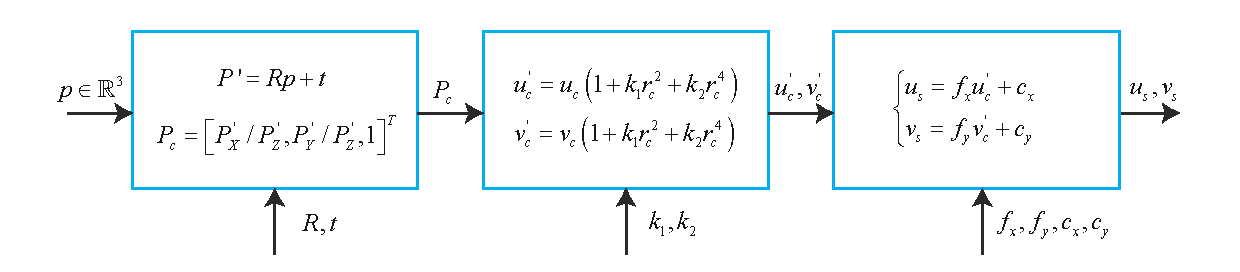
\includegraphics[width=1.0\textwidth]{backend1/calculationflow}
	\caption{计算流程示意图。左侧的$\bm{p}$是全局坐标系下的三维坐标点,右侧的$u_s,v_s$是该点在图像平面上的最终像素坐标。中间畸变模块中的$r_c^2=u_c^2 + v_c^2$。}
	\label{fig:calculationflow}
\end{figure}

现在,我们给出了它的详细参数化过程。具体地说,这里的$\bm{x}$指代此时相机的位姿,即外参$\bm{R}, \bm{t}$,它对应的李代数为$\bm{\xi}$。路标$\bm{y}$即这里的三维点$\bm{p}$,而观测数据则是像素坐标$\bm{z} \buildrel \Delta \over = [u_s, v_s]^T $。以最小二乘的角度来考虑,那么可以列写关于此次观测的误差:
\begin{equation}
\bm{e} = \bm{z} - h(\bm{\xi}, \bm{p}).
\end{equation}

然后,把其他时刻的观测量也考虑进来,我们可以给误差添加一个下标。设$\bm{z}_{ij}$为在位姿$\bm{\xi}_i$处观察路标$\bm{p}_j$产生的数据,那么整体的\textbf{代价函数}(Cost Function)为
\begin{equation}
\label{eq:BAcostfunction}
\frac{1}{2}\sum_{i=1}^m \sum_{j=1}^n \| \bm{e}_{ij} \|^2 = \frac{1}{2}\sum_{i=1}^m\sum_{j=1}^n \|
\bm{{z}}_{ij} - h(\bm{\xi}_{i},\bm{p}_j) \|^2 .
\end{equation}

对这个最小二乘进行求解,相当于对位姿和路标同时做了调整,也就是所谓的BA。接下来,我们会根据该目标函数和第6讲介绍的非线性优化内容,逐步深入探讨该模型的求解。

\subsection{BA的求解}
观察在上一节中的观测模型$h(\bm{\xi}, \bm{p})$,很容易判断该函数不是线性函数。所以我们希望使用6.2节介绍的一些非线性优化手段来优化它。根据非线性优化的思想,我们应该从某个初始值开始,不断地寻找下降方向$\Delta \bm{x}$来找到目标函数的最优解,即不断地求解增量方程\eqref{eq:minimize-deltax}中的增量$\Delta \bm{x}$。尽管误差项都是针对单个位姿和路标点的,但在整体BA目标函数上,我们必须把自变量定义成所有待优化的变量:
\begin{equation}
\bm{x} = [ \bm{\xi}_1, \ldots, \bm{\xi}_m, \bm{p}_1, \ldots, \bm{p}_n ]^\mathrm{T}.
\end{equation}

相应地,增量方程中的$\Delta \bm{x}$则是对整体自变量的增量。在这个意义下,当我们给自变量一个增量时,目标函数变为
\begin{equation}
\label{eq:tangentbundleindetail}
\frac{1}{2}\left\Vert f(\bm{x} + \Delta \bm{x}) \right\Vert ^2 \approx \frac{1}{2}\sum_{i=1}^{m}\sum_{j=1}^n \left\Vert \bm{e}_{ij} + \bm{F}_{ij} \Delta \bm{\xi}_{i} + \bm{E}_{ij} \Delta \bm{p}_j \right\Vert^2 .
\end{equation}

其中$\bm{F}_{ij}$表示整个代价函数在当前状态下对相机姿态的偏导数,而$\bm{E}_{ij}$表示该函数对路标点位置的偏导。我们曾在~\ref{sec:BA-vo1}~节中介绍了它们的具体形式,所以这里就不再展开推导了。现在,把相机位姿变量放在一起:
\begin{equation}
\bm{x}_c=[ \bm{\xi}_1, \bm{\xi}_2, \ldots, \bm{\xi}_m ]^\mathrm{T} \in \mathbb{R}^{6m},
\end{equation}
并把空间点的变量也放在一起:
\begin{equation}
\bm{x}_p=[ \bm{p}_1, \bm{p}_2, \ldots , \bm{p}_n ]^\mathrm{T}\in \mathbb{R}^{3n},
\end{equation}
那么,式\eqref{eq:tangentbundleindetail}可以简化表达如下:
\begin{equation}
\label{eq:BAleastsquare}
\frac{1}{2}
\left\Vert 
f(\bm{x}+ \Delta \bm{x} )
\right\Vert ^2 = 
\frac{1}{2} 
\left\Vert 
\bm{e} + \bm{F}\Delta \bm{x}_c + \bm{E} \Delta \bm{x}_p 
\right \Vert ^2 .
\end{equation}

需要注意的是,该式从一个由很多个小型二次项之和,变成了一个更整体的样子。这里的雅可比矩阵$\bm{E}$和$\bm{F}$必须是整体目标函数对整体变量的导数,它将是一个很大块的矩阵,而里头每个小分块,需要由每个误差项的导数$\bm{F}_{ij}$和$\bm{E}_{ij}$“拼凑”起来。然后,无论我们使用高斯牛顿法还是列文伯格—马夸尔特方法,最后都将面对增量线性方程:
\begin{equation}
\bm{H} \Delta \bm{x} = \bm{g}.
\end{equation}

\clearpage
根据第6讲的知识,我们知道高斯牛顿法和列文伯格—马夸尔特方法的主要差别在于,这里的$\bm{H}$是取$\bm{J}^\mathrm{T}\bm{J}$还是$\bm{J}^\mathrm{T}\bm{J}+ \lambda \bm{I}$的形式。由于我们把变量归类成了位姿和空间点两种,所以雅可比矩阵可以分块为
\begin{equation}
\bm{J}=[\bm{F} \ \bm{E}].
\end{equation}

那么,以高斯牛顿法为例,则$\bm{H}$矩阵为
\begin{equation}\label{eq:HessianMatrix}
\bm{H} = \bm{J}^\mathrm{T}\bm{J} =
\begin{bmatrix}
         \bm{F}^\mathrm{T}\bm{F}   &   \bm{F}^\mathrm{T}\bm{E}   \\ 
         \bm{E}^\mathrm{T}\bm{F}   &   \bm{E}^\mathrm{T}\bm{E}
\end{bmatrix} .
\end{equation}

当然在列文伯格—马夸尔特方法中我们也需要计算这个矩阵。不难发现,因为考虑了所有的优化变量,这个线性方程的维度将非常大,包含了所有的相机位姿和路标点。尤其是在视觉SLAM中,一幅图像就会提出数百个特征点,大大增加了这个线性方程的规模。如果直接对$\bm{H}$求逆来计算增量方程,由于矩阵求逆是复杂度为$O(n^3)$的操作\textsuperscript{\cite{Sueli2003}},这是非常消耗计算资源的。幸运的是,这里的$\bm{H}$矩阵是有一定的特殊结构的。利用这个特殊结构,我们可以加速求解过程。

\subsection{稀疏性和边缘化}
21世纪视觉SLAM的一个重要进展是认识到了矩阵$\bm{H}$的稀疏结构,并发现该结构可以自然、显式地用图优化来表示\textsuperscript{\cite{Kummerle2011, Polok2013}}。本节将详细讨论一下该矩阵稀疏结构。

$\bm{H}$矩阵的稀疏性是由雅可比矩阵$\bm{J}(\bm{x})$引起的。考虑这些代价函数当中的其中一个$\bm{e}_{ij}$。注意到,这个误差项只描述了在$\bm{\xi}_i$看到$\bm{p}_j$这件事,只涉及第$i$个相机位姿和第$j$个路标点,对其余部分的变量的导数都为0。所以该误差项对应的雅可比矩阵有下面的形式:
\begin{equation}
\bm{J}_{ij}(\bm{x}) = \left(
\bm{0}_{2 \times 6},...
\bm{0}_{2 \times 6},
\frac{\partial \bm{e}_{ij}}{\partial \bm{\xi}_i},
\bm{0}_{2 \times 6},...
\bm{0}_{2 \times 3},...
\bm{0}_{2 \times 3},
\frac{\partial \bm{e}_{ij}}{ \partial \bm{p}_j},
\bm{0}_{2 \times 3},...
\bm{0}_{2 \times 3} 
\right) .
\end{equation}

其中$\bm{0}_{2 \times 6}$表示维度为$2 \times 6$的$\bm{0}$矩阵,同理$\bm{0}_{2 \times 3}$也是一样。该误差项对相机姿态的偏导${\partial \bm{e}_{ij}}/{\partial \bm{\xi}_i}$维度为$2 \times 6$,对路标点的偏导${\partial \bm{e}_{ij}}/{\partial \bm{p}_j}$维度是$2 \times 3$。这个误差项的雅可比矩阵,除了这两处为非零块之外,其余地方都为零。这体现了该误差项与其他路标和轨迹无关的特性。那么,它对增量方程有何影响?$\bm{H}$矩阵为什么会产生稀疏性呢?

以\autoref{fig:sparse}~为例,我们设$\bm{J}_{ij}$只在$i,j$处有非零块,那么它对$\bm{H}$的贡献为$\bm{J}_{ij}^\mathrm{T} \bm{J}_{ij}$,具有图上所画的稀疏形式。这个$\bm{J}_{ij}^\mathrm{T} \bm{J}_{ij}$矩阵也仅有4个非零块,位于$(i,i), (i,j), (j,i), (j,j)$。对于整体的$\bm{H}$,由于:
\begin{equation}
\bm{H} = \sum_{i,j} \bm{J}_{ij}^\mathrm{T} \bm{J}_{ij},
\end{equation}
请注意$i$在所有相机位姿中取值,$j$在所有路标点中取值。我们把$\bm{H}$进行分块:
\begin{equation}
\label{eq:H-blocks}
\bm{H} = \left[ {\begin{array}{*{20}{c}}
	{{\bm{H}_{11}}}&{{\bm{H}_{12}}}\\
	{{\bm{H}_{21}}}&{{\bm{H}_{22}}}
	\end{array}} \right] .
\end{equation}

\begin{figure}[!htp]
	\centering
	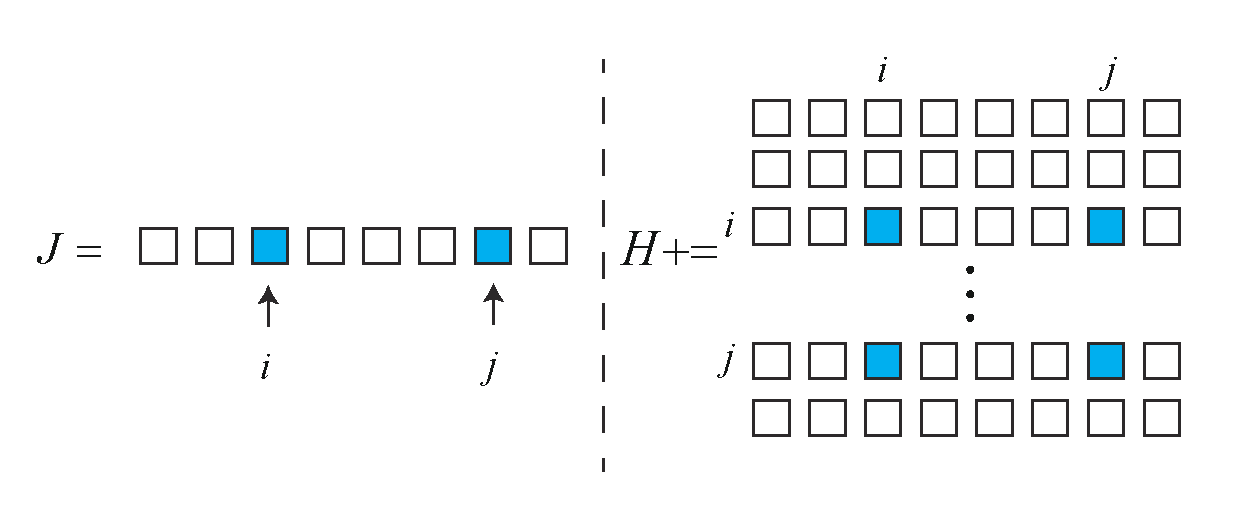
\includegraphics[width=1.0\textwidth]{backend1/sparse.pdf}
	\caption{当某个误差项$\bm{J}$具有稀疏性时,它对$\bm{H}$的贡献也具有稀疏形式。}
	\label{fig:sparse}
\end{figure}

这里$\bm{H}_{11}$只和相机位姿有关,而$\bm{H}_{22}$只和路标点有关。当我们遍历$i,j$时,以下事实总是成立的:
\begin{enumerate}
	\item 不管$i,j$怎么变,$\bm{H}_{11}$都是对角阵,只在$\bm{H}_{i,i}$处有非零块。
	\item 同理,$\bm{H}_{22}$也是对角阵,只在$\bm{H}_{j,j}$处有非零块。
	\item 对于$\bm{H}_{12}$和$\bm{H}_{21}$,它们可能是稀疏的,也可能是稠密的,视具体的观测数据而定。
\end{enumerate}

这显示了$\bm{H}$的稀疏结构。之后对线性方程的求解中,也正需要利用它的稀疏结构。也许读者还没有很好地领会这里的意思,我们举一个实例来直观说明它的情况。假设一个场景内有2个相机位姿($C_1,C_2$)和6个路标($P_1,P_2,P_3,P_4,P_5,P_6$)。这些相机和点云所对应的变量为$\bm{\xi}_i, i = 1,2$及$\bm{p}_j, j = 1,\cdots, 6$。相机$C_1$观测到路标$P_1,P_2,P_3,P_4$,相机$C_2$观测到路标$P_3,P_4,P_5,P_6$。我们把这个过程画成示意\autoref{fig:simplegraph}~。相机和路标以圆形节点表示。如果$i$相机能够观测到$j$点云,我们就在它们对应的节点连上一条边。

\begin{figure}[!htp]
	\centering
	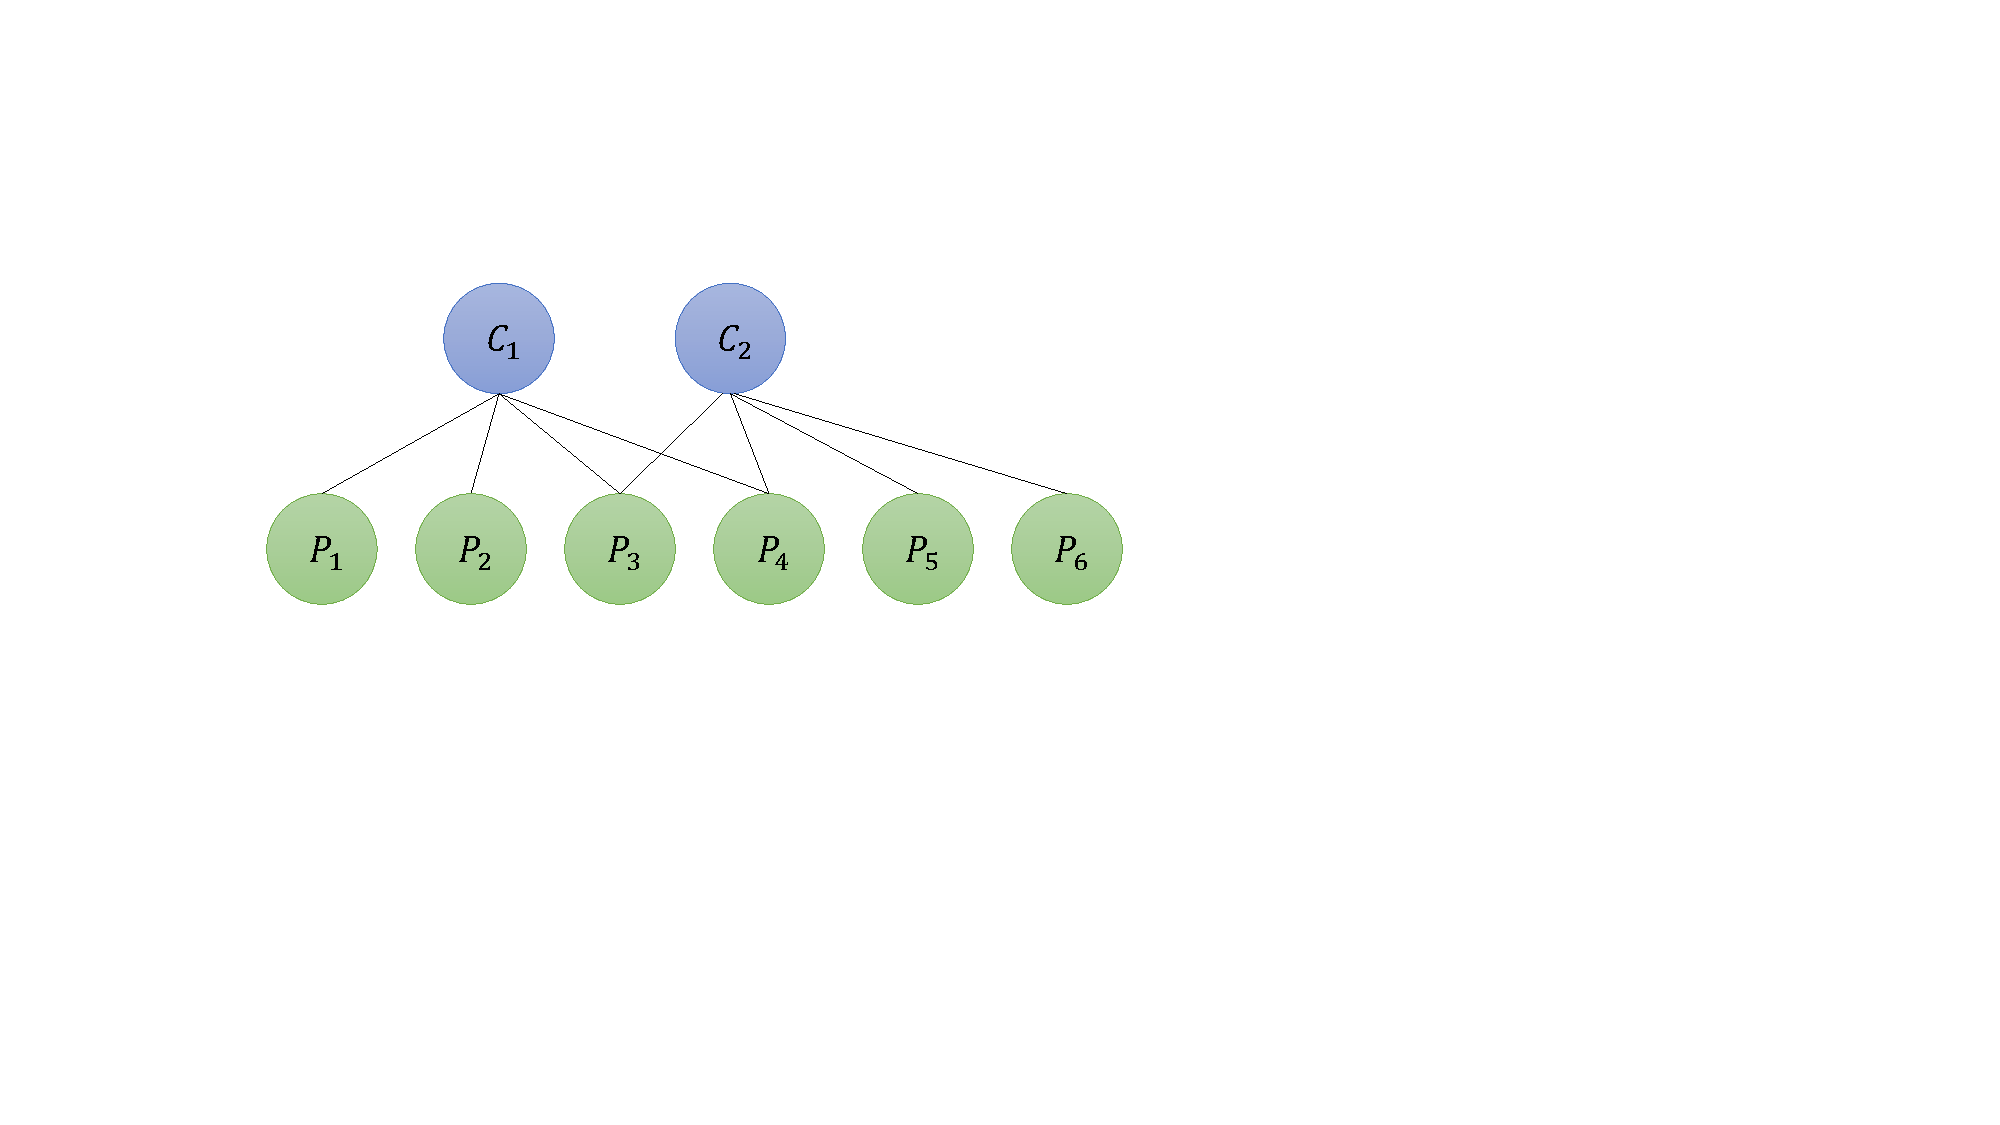
\includegraphics[width=0.8\textwidth]{backend1/simplegraph.pdf}
	\caption{点和边组成的示意图。该图显示相机$C_1$观测到了路标点$P_1,P_2,P_3,P_4$,相机$C_2$看到了$P_3$到$P_6$。}
	\label{fig:simplegraph}
\end{figure}

可以推出,场景下的BA目标函数应该是
\begin{equation}
\frac{1}{2}\left( \left\Vert \bm{e}_{11} \right\Vert^2 + 
\left\Vert \bm{e}_{12} \right\Vert^2 + 
\left\Vert \bm{e}_{13} \right\Vert^2 + 
\left\Vert \bm{e}_{14} \right\Vert^2 + 
\left\Vert \bm{e}_{23} \right\Vert^2 + 
\left\Vert \bm{e}_{24} \right\Vert^2 + 
\left\Vert \bm{e}_{25} \right\Vert^2 + 
\left\Vert \bm{e}_{26} \right\Vert^2 
\right).
\end{equation}

这里的$\bm{e}_{ij}$使用之前定义过的代价函数,即式\eqref{eq:BAcostfunction}。以$\bm{e}_{11}$为例,它描述了在$C_1$看到了$P_1$这件事,与其他的相机位姿和路标无关。令$\bm{J}_{11}$为$\bm{e}_{11}$所对应的雅可比矩阵,不难看出$\bm{e}_{11}$对相机变量$\bm{\xi}_2$和路标点$\bm{p}_2, \cdots, \bm{p}_6$的偏导都为0。我们把所有变量以$\bm{x} = \left( \bm{\xi}_1, \bm{\xi}_2, \bm{p}_1, \cdots, \bm{p}_2 \right)^\mathrm{T}$的顺序摆放,则有:
\begin{equation}
\bm{J}_{11} = \frac{\partial \bm{e}_{11}}{\partial \bm{x}}
= \left(
\frac{\partial \bm{e}_{11}}{\partial \bm{\xi}_1},
\bm{0}_{2\times 6},
\frac{\partial \bm{e}_{11}}{\partial \bm{p}_1},
\bm{0}_{2\times 3},
\bm{0}_{2\times 3},
\bm{0}_{2\times 3},
\bm{0}_{2\times 3},
\bm{0}_{2\times 3}
\right).
\end{equation}

为了方便表示稀疏性,我们用带有颜色的方块表示矩阵在该方块内有数值,其余没有颜色的区域表示矩阵在该处数值都为0。那么上面的$\bm{J}_{11}$则可以表示成\autoref{fig:jaobianrow}~所示图案。同理,其他的雅可比矩阵也会有类似的稀疏图案。

\begin{figure}[!htp]
	\centering
	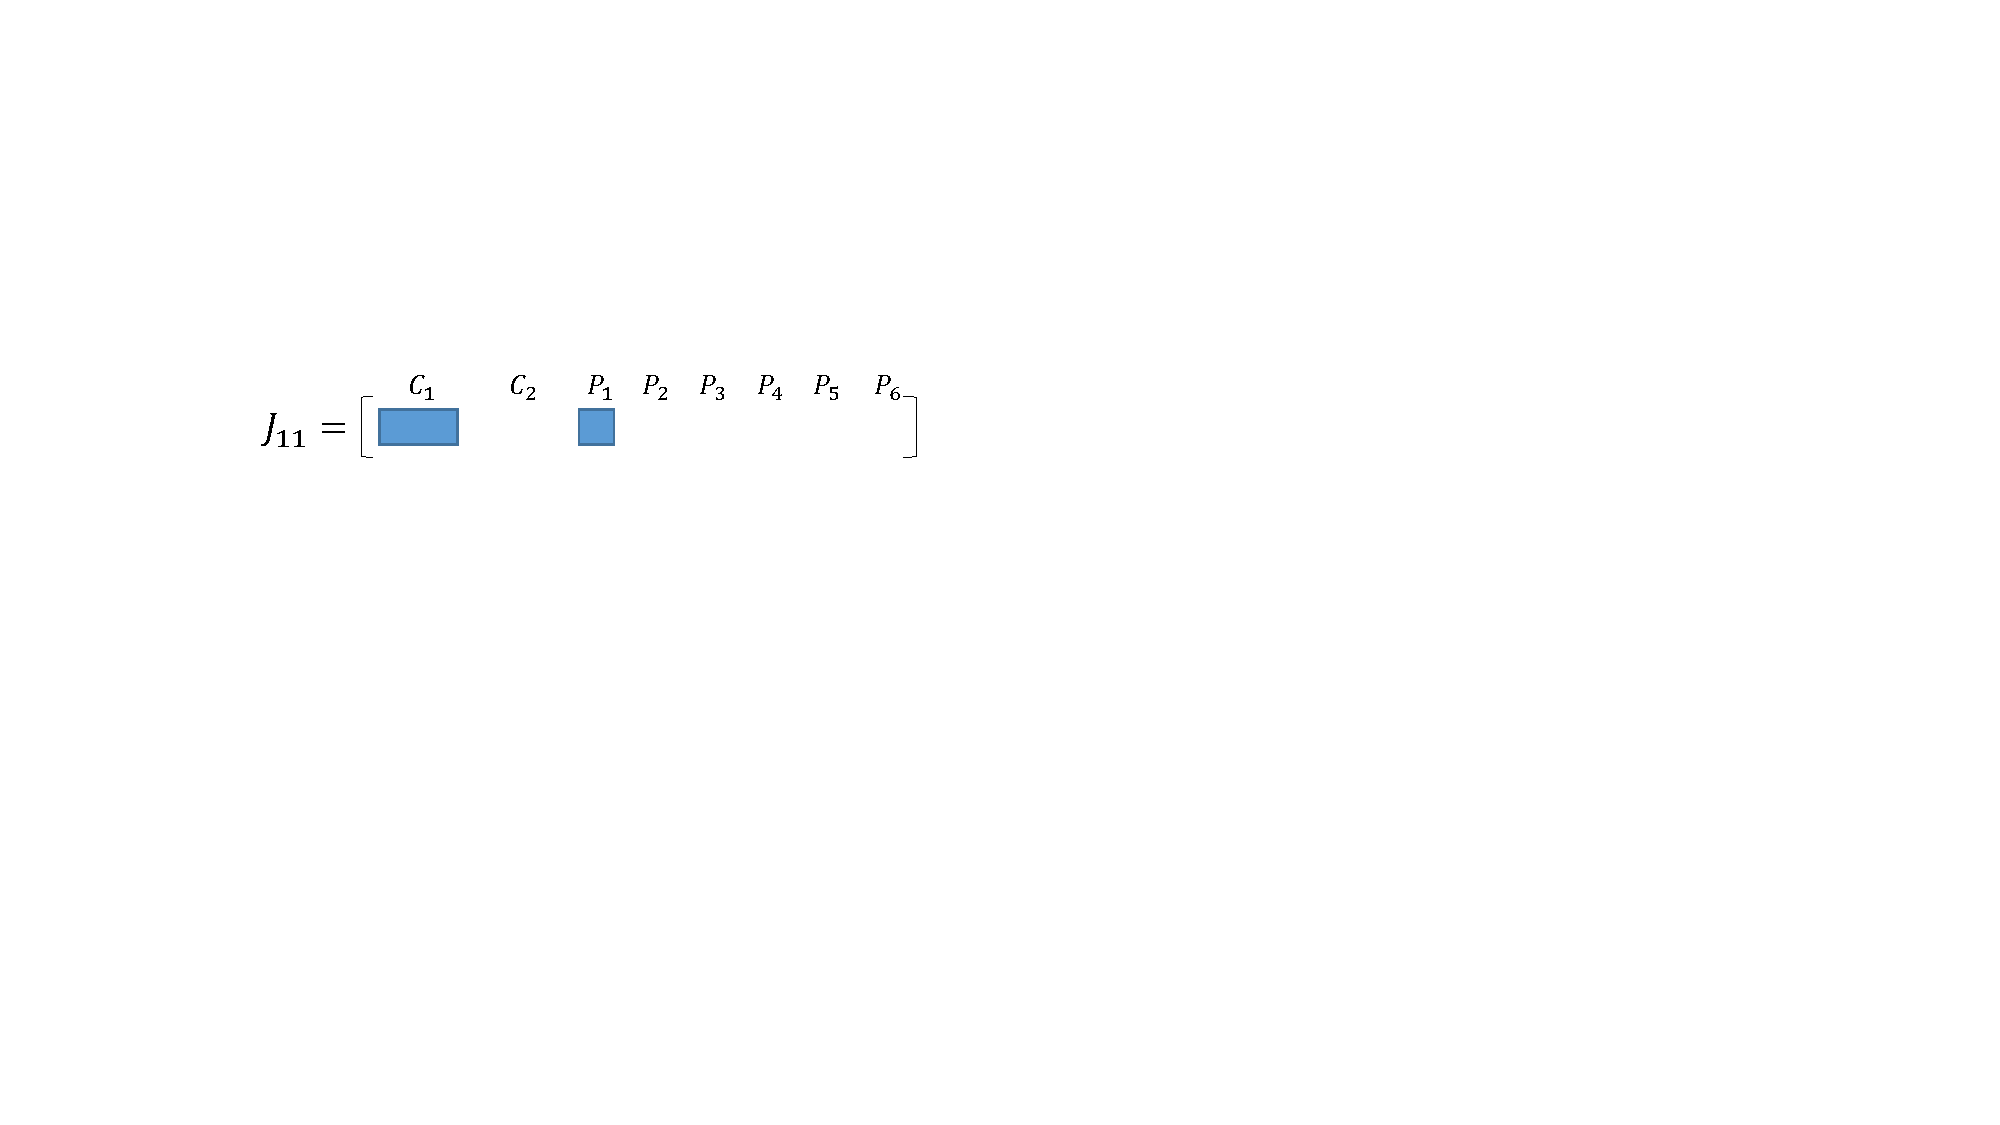
\includegraphics[width=0.8\textwidth]{backend1/Jacobianrow.pdf}
	\caption{$\bm{J}_{11}$矩阵的非零块分布图。上方的标记表示矩阵该列所对应的变量。由于相机参数维数比点云参数维数要大,所以$C_1$对应的矩阵块要比$P_1$对应的矩阵块宽一些。}
	\label{fig:jaobianrow}
\end{figure}

为了得到该目标函数对应的雅可比矩阵,我们可以将这些$\bm{J}_{ij}$按照一定顺序列为向量,那么整体雅可比矩阵及相应的$\bm{H}$矩阵的稀疏情况就如\autoref{fig:simplematrix}~所示。

\begin{figure}[!htp]
	\centering
	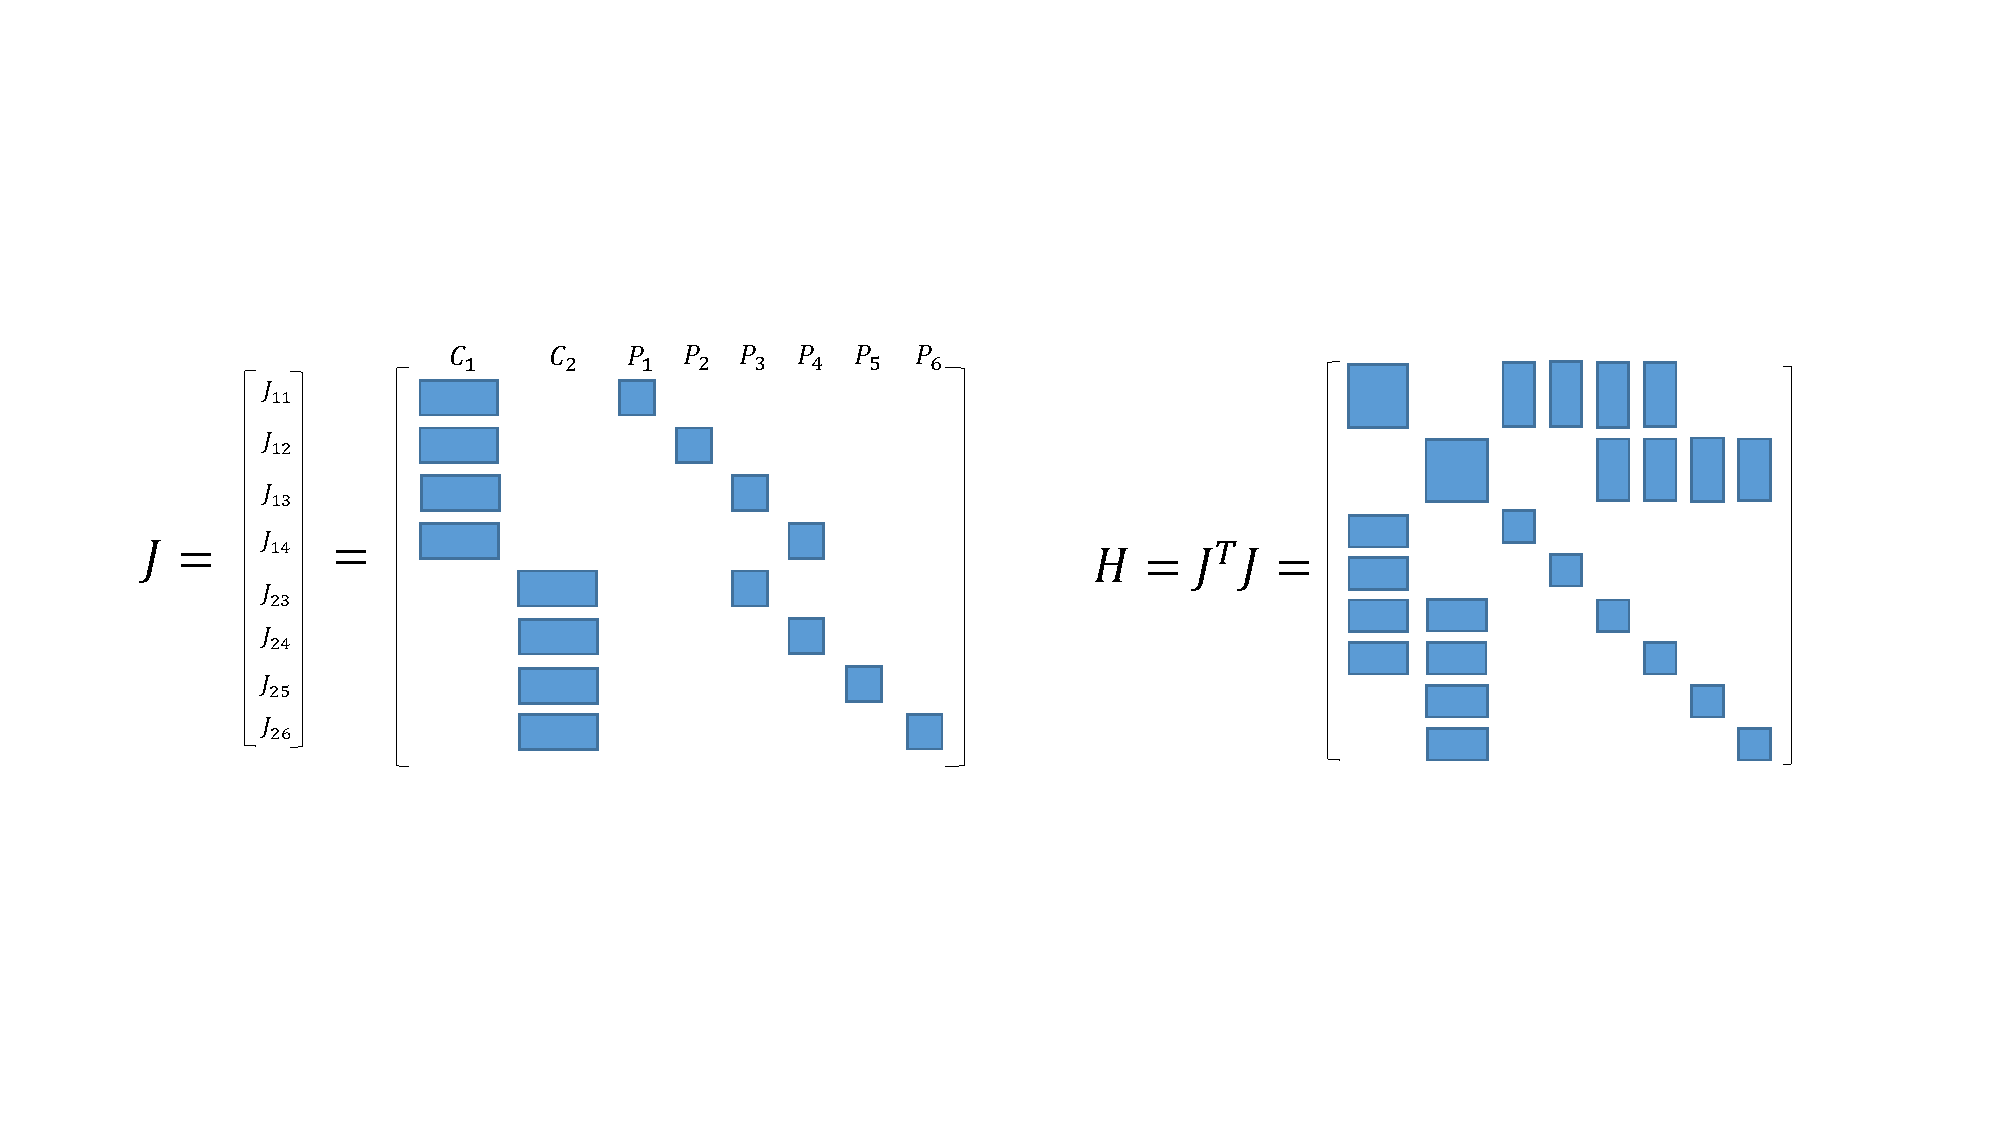
\includegraphics[width=1\textwidth]{backend1/simplematrix.pdf}
	\caption{雅可比矩阵的稀疏性(左)和$\bm{H}$矩阵的稀疏性(右),填色的方块表示矩阵在对应的矩阵块处有数值,其余没有颜色的部分表示矩阵在该处的数值始终为0。}
	\label{fig:simplematrix}
\end{figure}

\newpage
也许你已经注意到了,\autoref{fig:simplegraph}~对应的\textbf{邻接矩阵}(Adjacency Matrix)\footnote{所谓邻接矩阵是这样一种矩阵,它的第$i,j$个元素描述了节点$i$和$j$是否存在一条边。如果存在此边,设这个元素为1,否则设为0。}和上图中的$\bm{H}$矩阵,除了对角元素以外的其余部分有着完全一致的结构。事实上的确如此。上面的$\bm{H}$矩阵一共有$8 \times 8$个矩阵块,对于$\bm{H}$矩阵当中处于非对角线的矩阵块来说,如果该矩阵块非零,则其位置所对应的变量之间在图中会存在一条边,我们可以从\autoref{fig:matrixandgraph}~中清晰地看到这一点。所以,$\bm{H}$矩阵当中的非对角部分的非零矩阵块可以理解为其对应的两个变量之间存在联系,或者可以称之为约束。于是,我们发现图优化结构与增量方程的稀疏性存在着明显的联系。

\begin{figure}[!htp]
	\centering
	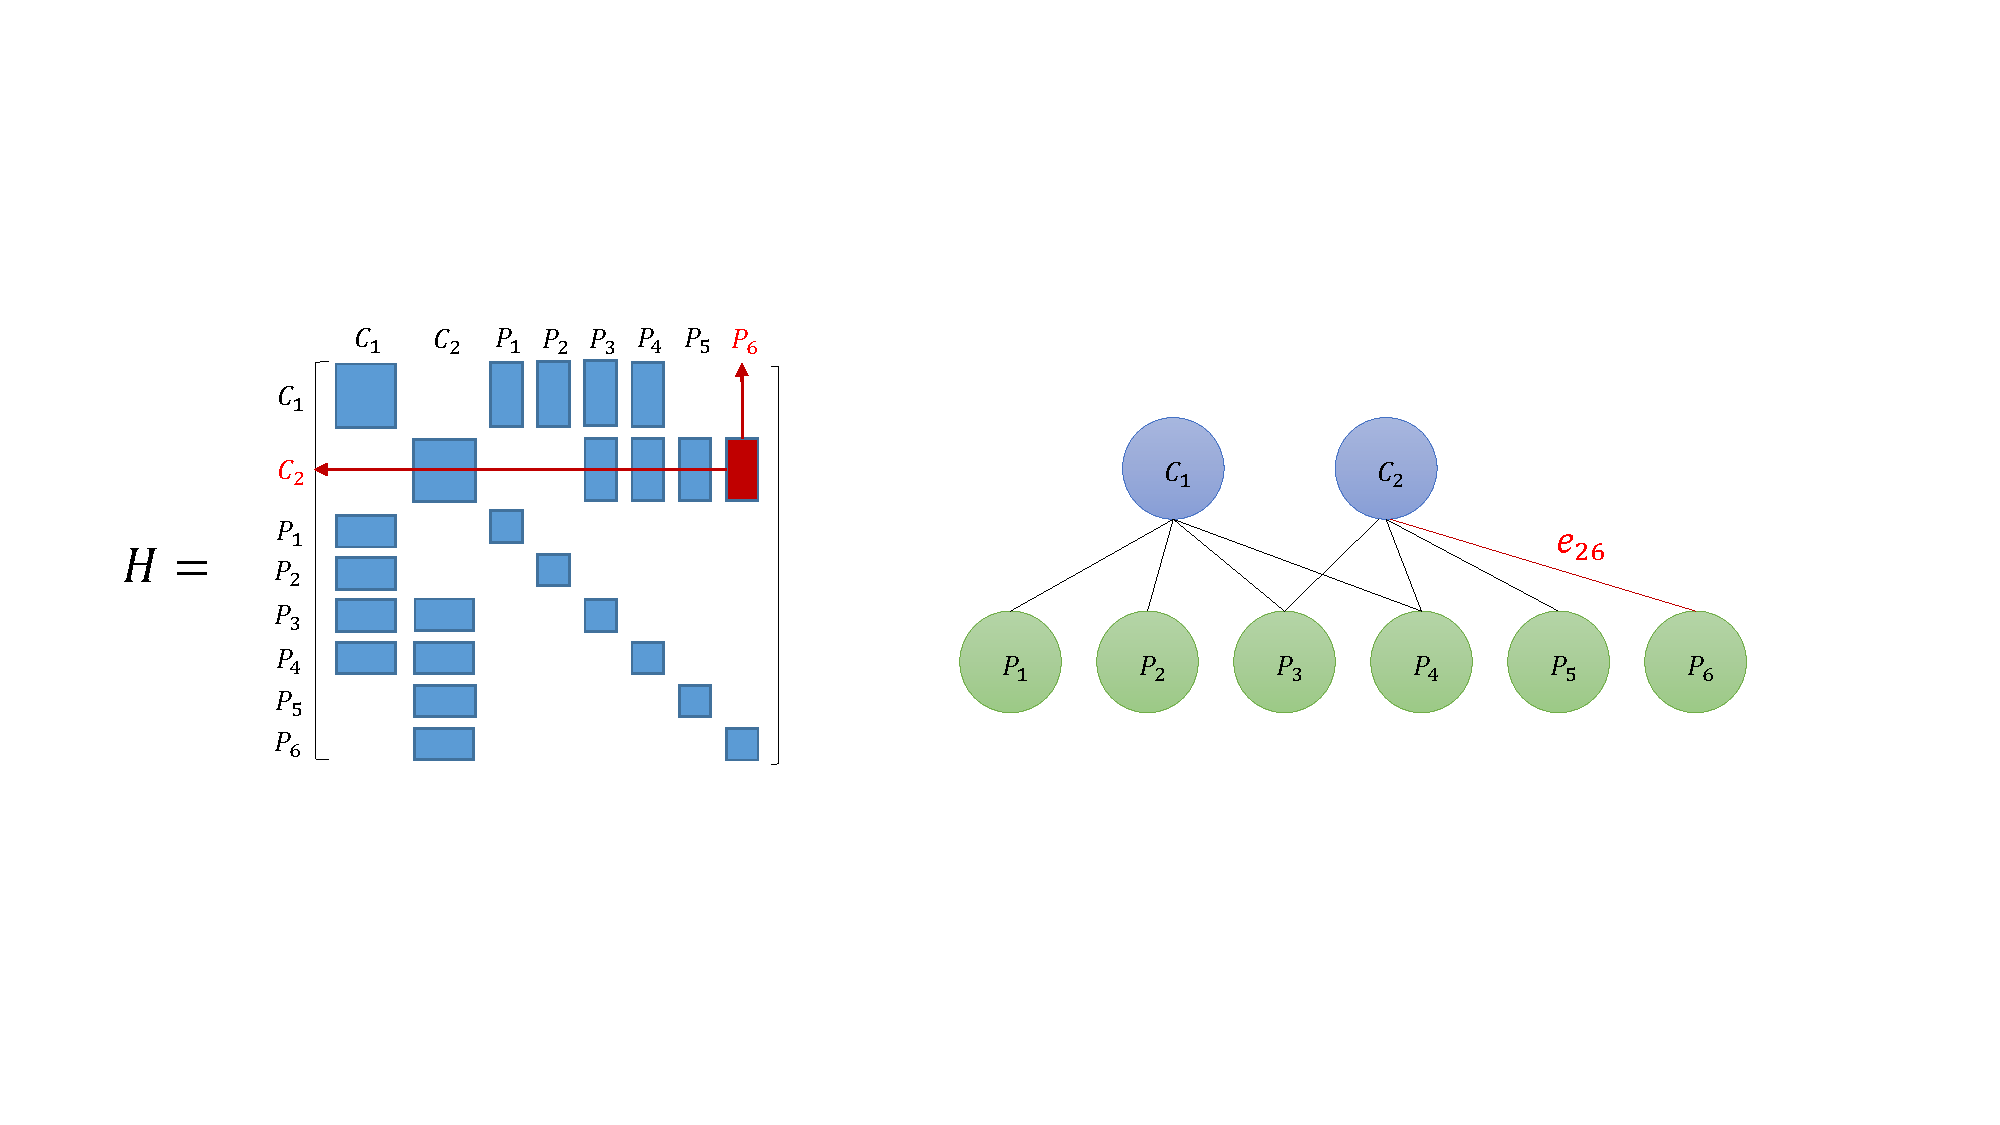
\includegraphics[width=1\textwidth]{backend1/matrixandgraph.pdf}
	\caption{$\bm{H}$矩阵中非零矩阵块和图中边的对应关系。如左图$\bm{H}$矩阵中右侧的红色矩阵块,表示在右图中其对应的变量$C_2$和$P_6$之间存在一条边$\bm{e}_{26}$。}
	\label{fig:matrixandgraph}
\end{figure}

现在考虑更一般的情况,假如我们有$m$个相机位姿,$n$个路标点。由于通常路标的数量远远多于相机,于是有$n \gg m$。由上面的推理可知,实际的$\bm{H}$矩阵会如\autoref{fig:BigHmatrix}~所示。它的左上角块显得非常小,而右下角的对角块占据了大量地方。除此之外,非对角部分则分布着散乱的观测数据。由于它的形状很像箭头,又称为箭头形(Arrow-like)矩阵\textsuperscript{\cite{Barfoot2016}}。同时,它也很像一把镐子,所以笔者也称其为镐形矩阵。

\begin{figure}[!ht]
	\centering
	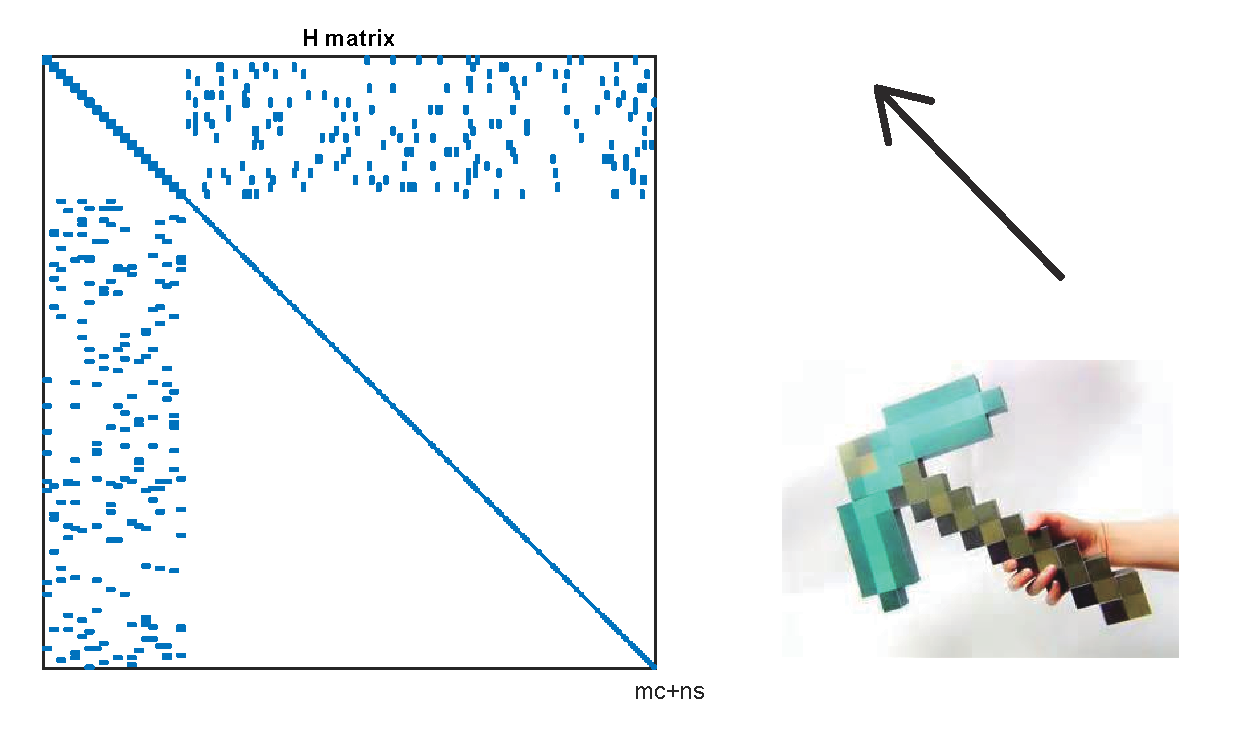
\includegraphics[width=0.7\textwidth]{backend1/BigHmatrix.pdf}
	\caption{一般情况下的$\bm{H}$矩阵。}
	\label{fig:BigHmatrix}
\end{figure}

对于具有这种稀疏结构的$\bm{H}$,线性方程$\bm{H} \Delta \bm{x}= \bm{g}$的求解会有什么不同呢?现实当中存在着若干种利用$\bm{H}$的稀疏性加速计算的方法,本节介绍视觉SLAM里一种最常用的手段:Schur消元。在SLAM研究中亦称为Marginalization(边缘化)。

仔细观察一下\autoref{fig:BigHmatrix},我们不难发现这个矩阵可以分成4个块,和式\eqref{eq:H-blocks}一致。左上角为对角块矩阵,每个对角块元素的维度与相机位姿的维度相同,且是一个对角块矩阵。右下角也是对角块矩阵,每个对角块的维度是路标的维度。非对角块的结构与具体观测数据相关。我们首先将这个矩阵按照\autoref{fig:MatrixSegmentation}所示的方式做区域划分,读者不难发现,这4个区域正好对应了公式\eqref{eq:HessianMatrix}中的4个矩阵块。为了后续分析方便,我们记这4个块为$\bm{B}, \bm{E}, \bm{E}^\mathrm{T}, \bm{C}$。

\begin{figure}[!ht]
	\centering
	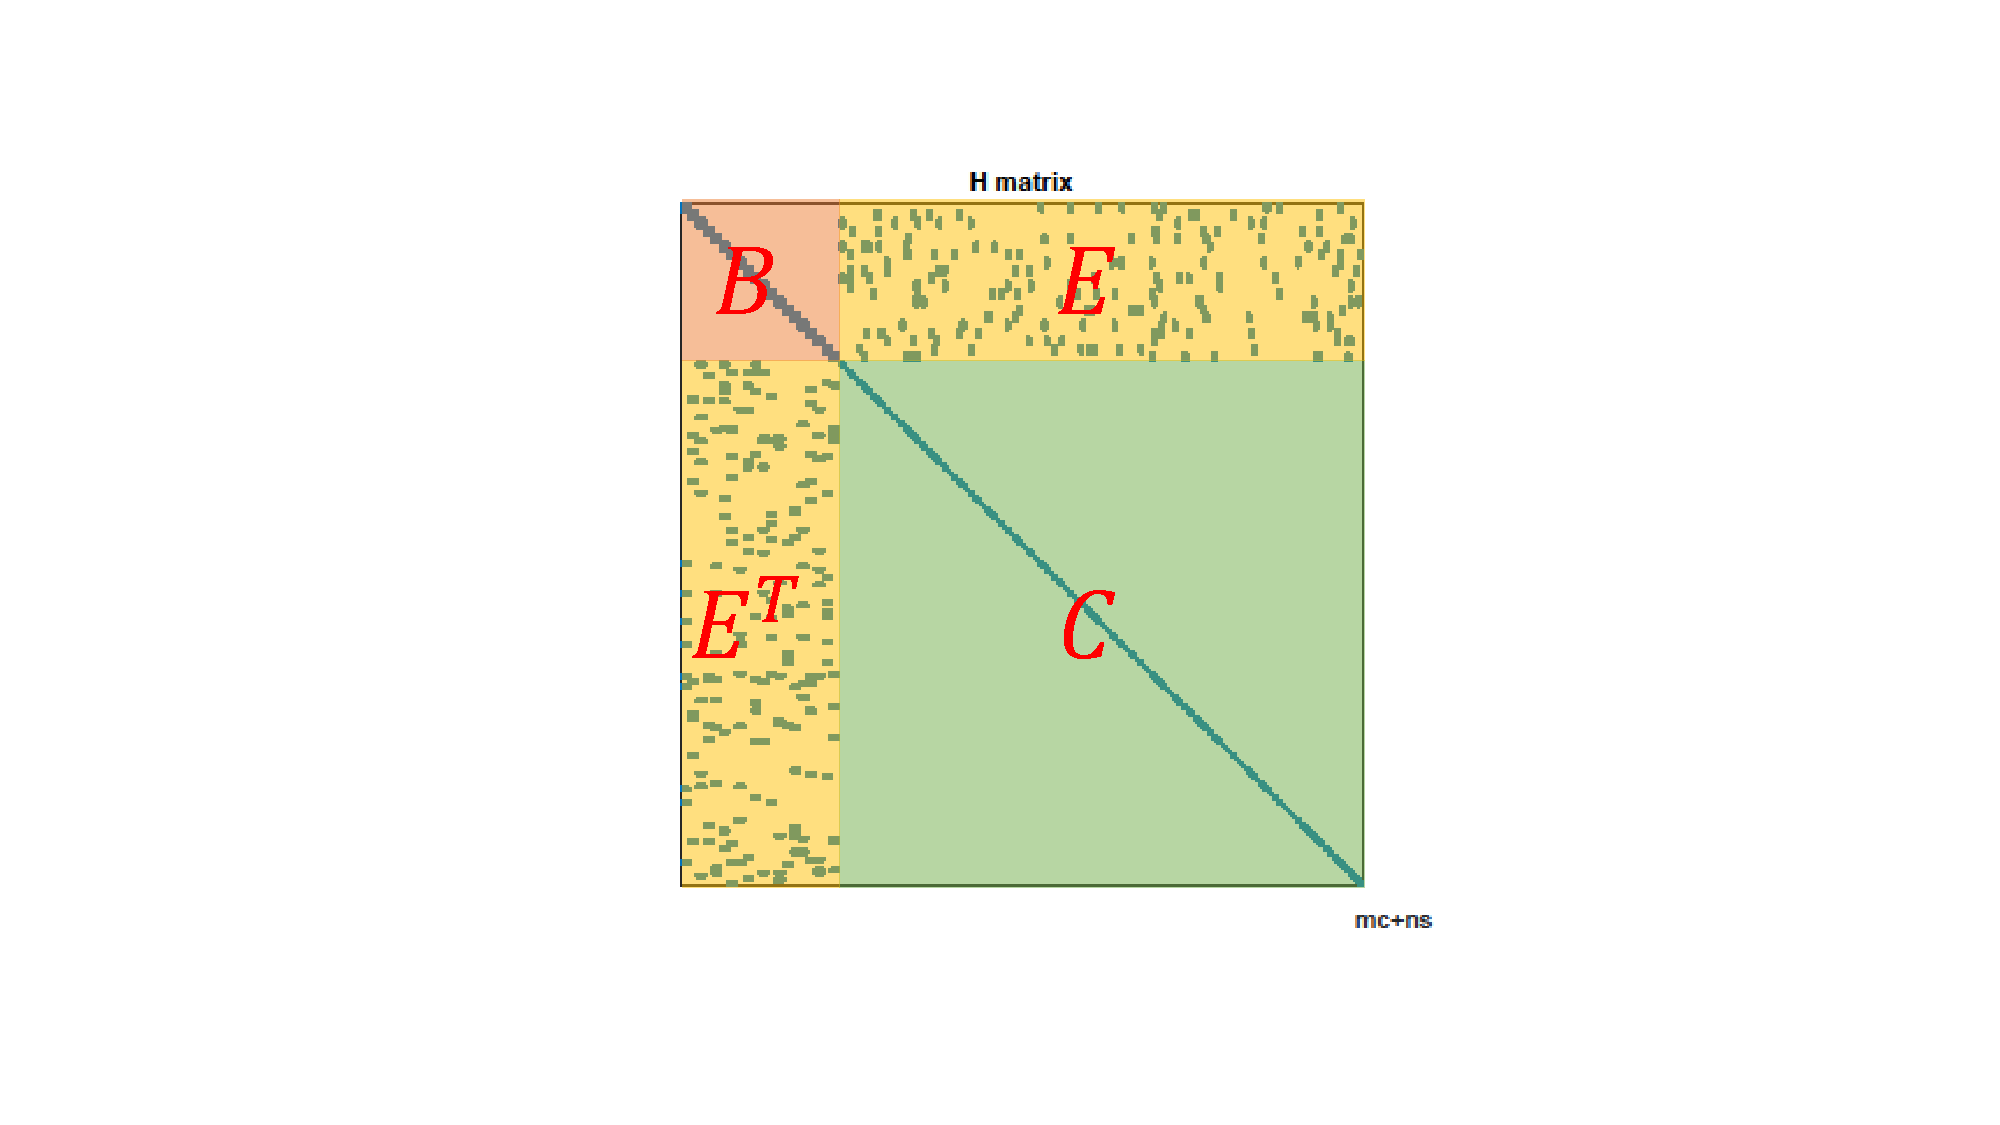
\includegraphics[width=0.5\textwidth]{backend1/MatrixSegmentation.pdf}
	\caption{$\bm{H}$矩阵的区域划分。}
	\label{fig:MatrixSegmentation}
\end{figure}

于是,对应的线性方程组也可以由$\bm{H\Delta x} = \bm{g}$变为如下形式:
\begin{equation}
\label{eq:linearequations}
 \left[ \begin{matrix}
\bm{B}   &   \bm{E} \\
\bm{E^\mathrm{T}} &   \bm{C}
\end{matrix}\right] 
\left[ \begin{array}{l}
\Delta \bm{x}_c \\
\Delta \bm{x}_p 
\end{array} \right] = 
\left[ \begin{array}{l}
\bm{v} \\
\bm{w} 
\end{array} \right].
\end{equation}

其中$\bm{B}$是对角块矩阵,每个对角块的维度和相机参数的维度相同,对角块的个数是相机变量的个数。由于路标数量会远远大于相机变量个数,所以$\bm{C}$往往也远大于$\bm{B}$。三维空间中每个路标点为三维,于是$\bm{C}$矩阵为对角块矩阵,每个块为$3 \times 3$矩阵。对角块矩阵求逆的难度远小于对一般矩阵的求逆难度,因为我们只需要对那些对角线矩阵块分别求逆即可。考虑到这个特性,我们对线性方程组进行高斯消元,目标是消去右上角的非对角部分$\bm{E}$,得:
\begin{equation}\label{eq:guasselimination}
\left[ \begin{matrix}
\bm{I}   &    -\bm{EC^{-1}} \\
\bm{0}	 &	  \bm{I}
\end{matrix}\right]
\left[ \begin{matrix}
\bm{B}   &   \bm{E} \\
\bm{E^\mathrm{T}} &   \bm{C}
\end{matrix}\right] 
\left[ \begin{array}{l}
\Delta \bm{x}_c \\
\Delta \bm{x}_p 
\end{array} \right] = 
\left[ \begin{matrix}
\bm{I}   &    -\bm{EC^{-1}}  \\
\bm{0}	 &	  \bm{I}
\end{matrix}
\right]
\left[ \begin{array}{l}
\bm{v} \\
\bm{w} 
\end{array} \right]  .
\end{equation}

整理,得:
\begin{equation}
\left[ \begin{matrix}
\bm{B} - \bm{E}\bm{C}^{-1}\bm{E}^\mathrm{T}	& 	\bm{0} \\
\bm{E}^\mathrm{T}							& 	\bm{C}
\end{matrix} \right]
\left[ \begin{array}{l}
\Delta \bm{x}_c \\
\Delta \bm{x}_p 
\end{array} \right] = 
\left[\begin{array}{l}
\bm{v} - \bm{E}\bm{C}^{-1}\bm{w}  \\
\bm{w}
\end{array}\right].
\end{equation}

经过消元之后,方程组第一行变成和$\Delta \bm{x}_p$无关的项。单独把它拿出来,得到关于位姿部分的增量方程:
\begin{equation}\label{eq:marginalization}
\left[ 
\bm{B} - \bm{E}\bm{C}^{-1}\bm{E}^\mathrm{T}
\right]
\Delta \bm{x}_c  = 
\bm{v} - \bm{E}\bm{C}^{-1}\bm{w} .
\end{equation}

这个线性方程的维度和$\bm{B}$矩阵一样。我们的做法是先求解这个方程,然后把解得的$\Delta \bm{x}_c$代入到原方程,然后求解$\Delta \bm{x}_p$。这个过程称为\textbf{Marginalization}\textsuperscript{\cite{Sibley2010}},或者\textbf{Schur消元}(Schur Elimination)。相比于直接解线性方程的做法,它的优势在于:

\begin{enumerate}
	\item 在消元过程中,由于$\bm{C}$为对角块,所以$\bm{C}^{-1}$容易解出。
	\item 求解了$\Delta \bm{x}_c$之后,路标部分的增量方程由$\Delta \bm{x}_p = \bm{C}^{-1} (\bm{w} - \bm{E}^\mathrm{T} \Delta \bm{x}_c)$给出。这依然用到了$\bm{C}^{-1}$易于求解的特性。
\end{enumerate}

于是,边缘化的主要计算量在于求解式\eqref{eq:marginalization}。关于这个方程,我们能说的就不多了。它仅是一个普通的线性方程,没有特殊的结构可以利用。我们将此方程的系数记为$\bm{S}$,它的稀疏性如何呢?\autoref{fig:marginalization}显示了进行Schur消元之后的一个$\bm{S}$实例,可以看到它的稀疏性是不规则的。

\clearpage
\begin{figure}[!ht]
	\centering
	\includegraphics[width=0.5\textwidth]{backend1/marginalization.pdf}
	\caption{对$\bm{H}$矩阵进行Schur消元后$\bm{S}$矩阵的稀疏状态。}
	\label{fig:marginalization}
\end{figure}

前面说到,$\bm{H}$矩阵的非对角块处的非零元素对应着相机和路标的关联。那么,进行了Schur消元后$\bm{S}$的稀疏性是否具有物理意义呢?答案是肯定的。此处我们不加证明地说,$\bm{S}$矩阵的非对角线上的非零矩阵块,表示了该处对应的两个相机变量之间存在着共同观测的路标点,有时候称为共视(Co-visibility)。反之,如果该块为零,则表示这两个相机没有共同观测。例如\autoref{fig:marginalizationanalysis}~所示的稀疏矩阵,左上角前$4 \times 4$个矩阵块可以表示对应的相机变量$C_1,C_2,C_3,C_4$之间有共同观测。

\begin{figure}[!htp]
	\centering
	\includegraphics[width=0.8\textwidth]{backend1/marginalizationanalysis.pdf}
	\caption{以$\bm{S}$矩阵中前$4 \times 4$个矩阵块为例,这个区域当中的矩阵块$\bm{S}_{14}, \bm{S}_{24}$不为零,表示相机$C_4$和相机$C_1$、$C_2$之间有共同观测点;而$S_{34}$为零则表示$C_3$和$C_4$之间没有共同观测的路标。}
	\label{fig:marginalizationanalysis}
\end{figure}
\clearpage
于是,$\bm{S}$矩阵的稀疏性结构当取决于实际观测的结果,我们无法提前预知。在实践当中,例如ORB-SLAM\textsuperscript{\cite{Mur-Artal2015}}中的Local Mapping 环节,在做BA的时候刻意选择那些具有共同观测的帧作为关键帧,在这种情况下Schur消元后得到的$\bm{S}$就是稠密矩阵。不过,由于这个模块并不是实时执行,所以这种做法也是可以接受的。但是在另一些方法里面,例如DSO\textsuperscript{\cite{Engel2016}}、OKVIS\textsuperscript{\cite{Leutenegger2015}}等,它们采用了滑动窗口方法(Sliding Window)。这类方法对每一帧都要求做一次BA来防止误差的累积,因此它们也必须采用一些技巧来保持$\bm{S}$矩阵的稀疏性。读者如果希望能够更加深入这一块,可以参考它们的论文。这里就不谈这些过于细节的事情了。

从概率角度来看,我们称这一步为边缘化,是因为我们实际上把求$(\Delta \bm{x}_c, \Delta \bm{x}_p)$的问题,转化成了先求$\Delta \bm{x}_c$,再求$\Delta \bm{x}_p$的过程。这一步相当于做了条件概率展开:
\begin{equation}
P( \bm{x}_c, \bm{x}_p ) = P( \bm{x}_c ) \cdot P(\bm{x}_p | \bm{x}_c ).
\end{equation}

结果是求出了关于$\bm{x}_c$的边缘分布,故称边缘化。在前面讲的边缘化过程中,我们实际把所有的路标点都给边缘化了。根据实际情况,我们也能选择一部分进行边缘化。同时,Schur消元只是实现边缘化的其中一种方式,同样可以使用Cholesky分解进行边缘化。

读者可能会继续问,在进行了Schur消元后,我们还需要求解线性方程组\eqref{eq:marginalization}。对它的求解是否还有什么技巧呢?很遗憾,这部分就属于传统的矩阵数值求解了,通常是用分解来计算的。不管采用哪种求解办法,我们都建议利用$\bm{H}$的稀疏性进行Schur消元。不光是因为这样可以提高速度,也因为消元后的$\bm{S}$矩阵的条件数往往比之前的$\bm{H}$矩阵要小。Schur消元也并不意味着将所有路标消元,将相机变量消元也是SLAM当中采用的手段。

%\subsection{稀疏线性方程组求解}
%在进行了Schur消元后,我们还需要求解线性方程组\eqref{eq:marginalization}。我们将这个式子简写成公式\eqref{eq:reducedBundleAdjustment}。其中$\bm{S}$是维数为$mc \times mc$的半正定对称矩阵,$\bm{p}$是维数为$mc \times 1$维的向量。
%
%\begin{equation}\label{eq:reducedBundleAdjustment}
%\bm{S}\Delta \bm{x}_c = \bm{p}
%\end{equation}
%
%读者也许会觉得此处很简单,对$\bm{S}$求逆或者违逆就可以得到这个方程的解\eqref{eq:reducedBundleAdjustment},这么做理论上的确可以,但是如果你仔细思考一下也会发现,尽管我们这里得到的$\bm{S}$矩阵相比之前的$\bm{H}$来说已经大幅度缩小了维度,但求逆(或者违逆)依然是个计算量非常大的计算。其实不光是SLAM,其余领域的工程计算也很少会去用求逆(或者伪逆)这类思路去解决。
%
%由于解决线性方程组的方法五花八门,这里并不会将它们拿出来一一介绍。通常在一般情况下,求解线性方程组的方式是LU分解,但在这里,由于我们的$\bm{S}$矩阵是对称的半正定矩阵,可以采用更快速的手段来做。在SLAM或者SFM当中,常见的方法包括Cholesky分解或者$LDL^T$分解。其中Cholesky用来分解正定矩阵,$LDL^T$用来分解对称矩阵,因此这两者的选择主要是看$\bm{S}$矩阵所具有的特点。由于在SLAM里我们通常会让$\bm{S}$矩阵正定,我们接下来会对正定矩阵情况下采用的Cholesky分解方法重点介绍。你也许会好奇为何矩阵的分解会加速这个线性方程组的求解,因此在这之前,我们先回顾一下针对三角矩阵的线性方程组求解方法:
%
%假设$\bm{L}$矩阵是维度为$n \times n$的下三角矩阵,并且对角线上的元素非零。$\bm{b}$是维度为$n \times 1$的向量,那么线性方程组$\bm{Lx=b}$展开可以得到下面形式:
%$$\begin{array}{*{20}{c}}
%\begin{array}{l}
%{L_{11}}{x_1}\\
%{L_{21}}{x_1} + {L_{22}}{x_2}\\
%\vdots \\
%\vdots \\
%{L_{n1}}{x_1} + {L_{n2}}{x_2} +  \cdots  \cdots {L_{nn}}{x_n}
%\end{array}&\begin{array}{l}
%= {b_1}\\
%= {b_2}\\
%\vdots \\
%\vdots \\
%= {b_n}
%\end{array}
%\end{array}	$$
%
%此时,我们可以从第一行直接求出$x_1$,接着代入第二行${L_{21}}{x_1} + {L_{22}}{x_2} $求出$x_2$,依次类推可以得到最后的$x_n$。整个过程从$x_1$一直求出$x_n$,这个过程被称之为\textbf{顺向代入}(forward substitution)。其伪代码可以如下表示:
%
%\begin{algorithm}[h]
%	\caption{(顺向代入法)}
%	\label{alg:forwardsubstitution}
%	\begin{algorithmic}[1]
%		\REQUIRE
%		$\bm{L}$: 实数下三角矩阵,对角线元素非零;
%		$\bm{b}$: 实数向量;
%		$n$: $\bm{L}$的维度;
%		\FOR{$i=1$ to $n$ }
%		
%		\STATE $x_i = (b_i - \sum_{k=0}^{i-1}{L_{ik}x_k})/L_{ii}$;
%		
%		\ENDFOR
%		
%		\RETURN
%		$\bm{x}$
%	\end{algorithmic}
%\end{algorithm}
%
%当然,当$\bm{L}$为一个上三角矩阵的时候,则对应的代入顺序则是先求出最后一项$x_n$,然后一直代入最后求出$x_1$。这个过程被成为\textbf{逆向代入法}(back substitution)。对应的伪代码则如下:
%
%\begin{algorithm}[h]
%	\caption{(逆向代入法)}
%	\label{alg:backsubstitution}
%	\begin{algorithmic}[1]
%		\REQUIRE
%		$\bm{L}$: 实数下三角矩阵,对角线元素非零;
%		$\bm{b}$: 实数向量;
%		$n$: $\bm{L}$的维度;
%		\FOR{$i=n$ to $1$ }
%		
%		\STATE $x_i = (b_i - \sum_{k=i}^{n}{L_{ik}x_k})/L_{ii}$;
%		
%		\ENDFOR
%		
%		\RETURN
%		$\bm{x}$
%	\end{algorithmic}
%\end{algorithm}
%
%基于三角矩阵的这类优秀特性,在解决线性方程组的时候先将其分解为三角矩阵是常用的求解方法之一。我们要介绍的Cholesky分解是将一个正定矩阵$\bm{S}$分解为$\bm{S} = \bm{L}\bm{L^T}$的形式,当$\bm{L}$矩阵对角线元素为正数的时候,分解结果具有唯一性。Cholesky分解的操作也非常简单,即从对角线元素开始,依次将对角线元素下方的每一列递推完成:
%
%\begin{algorithm}[h]
%	\caption{(Cholesky 分解)}
%	\label{alg:CholeskyDecomposition}
%	\begin{algorithmic}[1]
%		\REQUIRE
%		$\bm{S}$: 实数正定矩阵;
%		$n$: 正定矩阵$\bm{S}$的维度;
%		\FOR{$j=1$ to $n$}
%		
%		\STATE $\bm{L}_{jj} = \sqrt{\bm{S}_{jj} - \sum_{k=1}^{j-1}{L_{jk}^2}}$;
%		
%		\FOR{$i=j+1$ to $n$}
%		\STATE $\bm{L}_{ij} = \frac{1}{\bm{L}_{jj}}(\bm{S}_{ij} - \sum_{k=1}^{j-1}{\bm{L}_{ik}\bm{L}_{jk}})$;
%		\ENDFOR
%		
%		\ENDFOR
%		\RETURN
%		$\bm{L}$ 
%	\end{algorithmic}
%\end{algorithm}
%
%容易看出,该算法的复杂度为$O(n^3)$,其中$n$为矩阵的维度。在对\eqref{eq:reducedBundleAdjustment}进行了Cholesky分解之后,我们需要求解的线性方程组则变成了$\bm{LL^T}\Delta \bm{x}_c = \bm{p}$。为了充分利用三角矩阵求解带来的便利,我们将$\bm{L^T} \Delta \bm{x}_c$ 这个向量记作$\bm{y}$。这样一来,我们可以首先求解$\bm{Ly=b}$来得到$\bm{y}$,接着再次借助三角矩阵求解带来的便利来求$\bm{L^T} \Delta \bm{x}_c = \bm{y}$,从而得到最终的$\Delta \bm{x}_c $。这样我们不难总结出,使用Cholesky分解求解线性方程组的流程大致如下:
%
%\begin{algorithm}[h]
%	\caption{(Cholesky 分解求解线性方程组)}
%	\label{alg:CholeskyLinearsolver}
%	\begin{algorithmic}[1]
%		\REQUIRE
%		$\bm{S}$: 实数正定矩阵
%		$n$: 正定矩阵$\bm{S}$的维度
%		$\bm{b}$: 维数为$n \times 1$的实数向量
%		\STATE 使用(\ref{alg:CholeskyDecomposition})将矩阵$\bm{S}$进行Cholesky分解,得到其对应的下三角矩阵$\bm{L}$;
%		
%		\STATE 使用顺向代入法(\ref{alg:forwardsubstitution})求解线性方程组$\bm{Ly = b}$,得到向量$\bm{y}$;
%		
%		\STATE 使用逆向代入法(\ref{alg:backsubstitution})求解线性方程组$\bm{L^Tx = y}$,得到向量$\bm{x}$;
%	
%		\RETURN
%		$\bm{x}$ 
%	\end{algorithmic}
%\end{algorithm}
%
%对于半正定的矩阵来说,通常的做法就是在加上一个比较小的对角矩阵,然后让其可逆。当然我们还需要考虑一类情况,那就是$\bm{S}$矩阵为稀疏矩阵的时候,这就会涉及到稀疏矩阵线性方程组的求解问题。稀疏性会给SLAM提供很大的便利,不光是从算法速度上,还是从算法占用的内存空间上。稀疏矩阵的存储有很多种,其中最简单的就是仅仅只保存非零元素所在的行列以及自身的数值,最后放在一个Hash表里进行管理。但稀疏矩阵的数据结构会根据算法所需进行定制。
%
%好在这些底层的数学内容,现有的很多算法库都已经做的挺完整,比如CHOLMOD\cite{chen2008algorithm},CSparse\cite{davis2005csparse}这类高效的Cholesky分解算法库已经用在广泛的工业界和学术界,连著名的软件MATLAB也是调用的它,也有Suitsparse\cite{davis2014suitesparse}这类算法库集成了针对稀疏矩阵的各种分解的高效算法,因此绝大多数人都可以忽略这些理论上的细节,选择去熟悉这些算法库的调用也是可取的。
%
%但为了方便读者熟悉各类SLAM的前沿理论研究,笔者还是得对稀疏矩阵进行简要的描述。在研究稀疏矩阵的分解操作时,有个概念叫做\textbf{填充}(fill-in)。这个概念指的是在稀疏矩阵原本为0的位置当中,其中某些位置在其分解后变成了带有数值的元素。比如下面对我们对箭头型矩阵直接进行Cholesky分解,就会出现\autoref{fig:ArrowMatrix}这样的情况。我们可以发现,再进行了Cholesky分解后,箭头矩阵那些原本为零的地方几乎全被\textbf{填充}了。
%
%\begin{figure}[!htp]
%	\centering
%	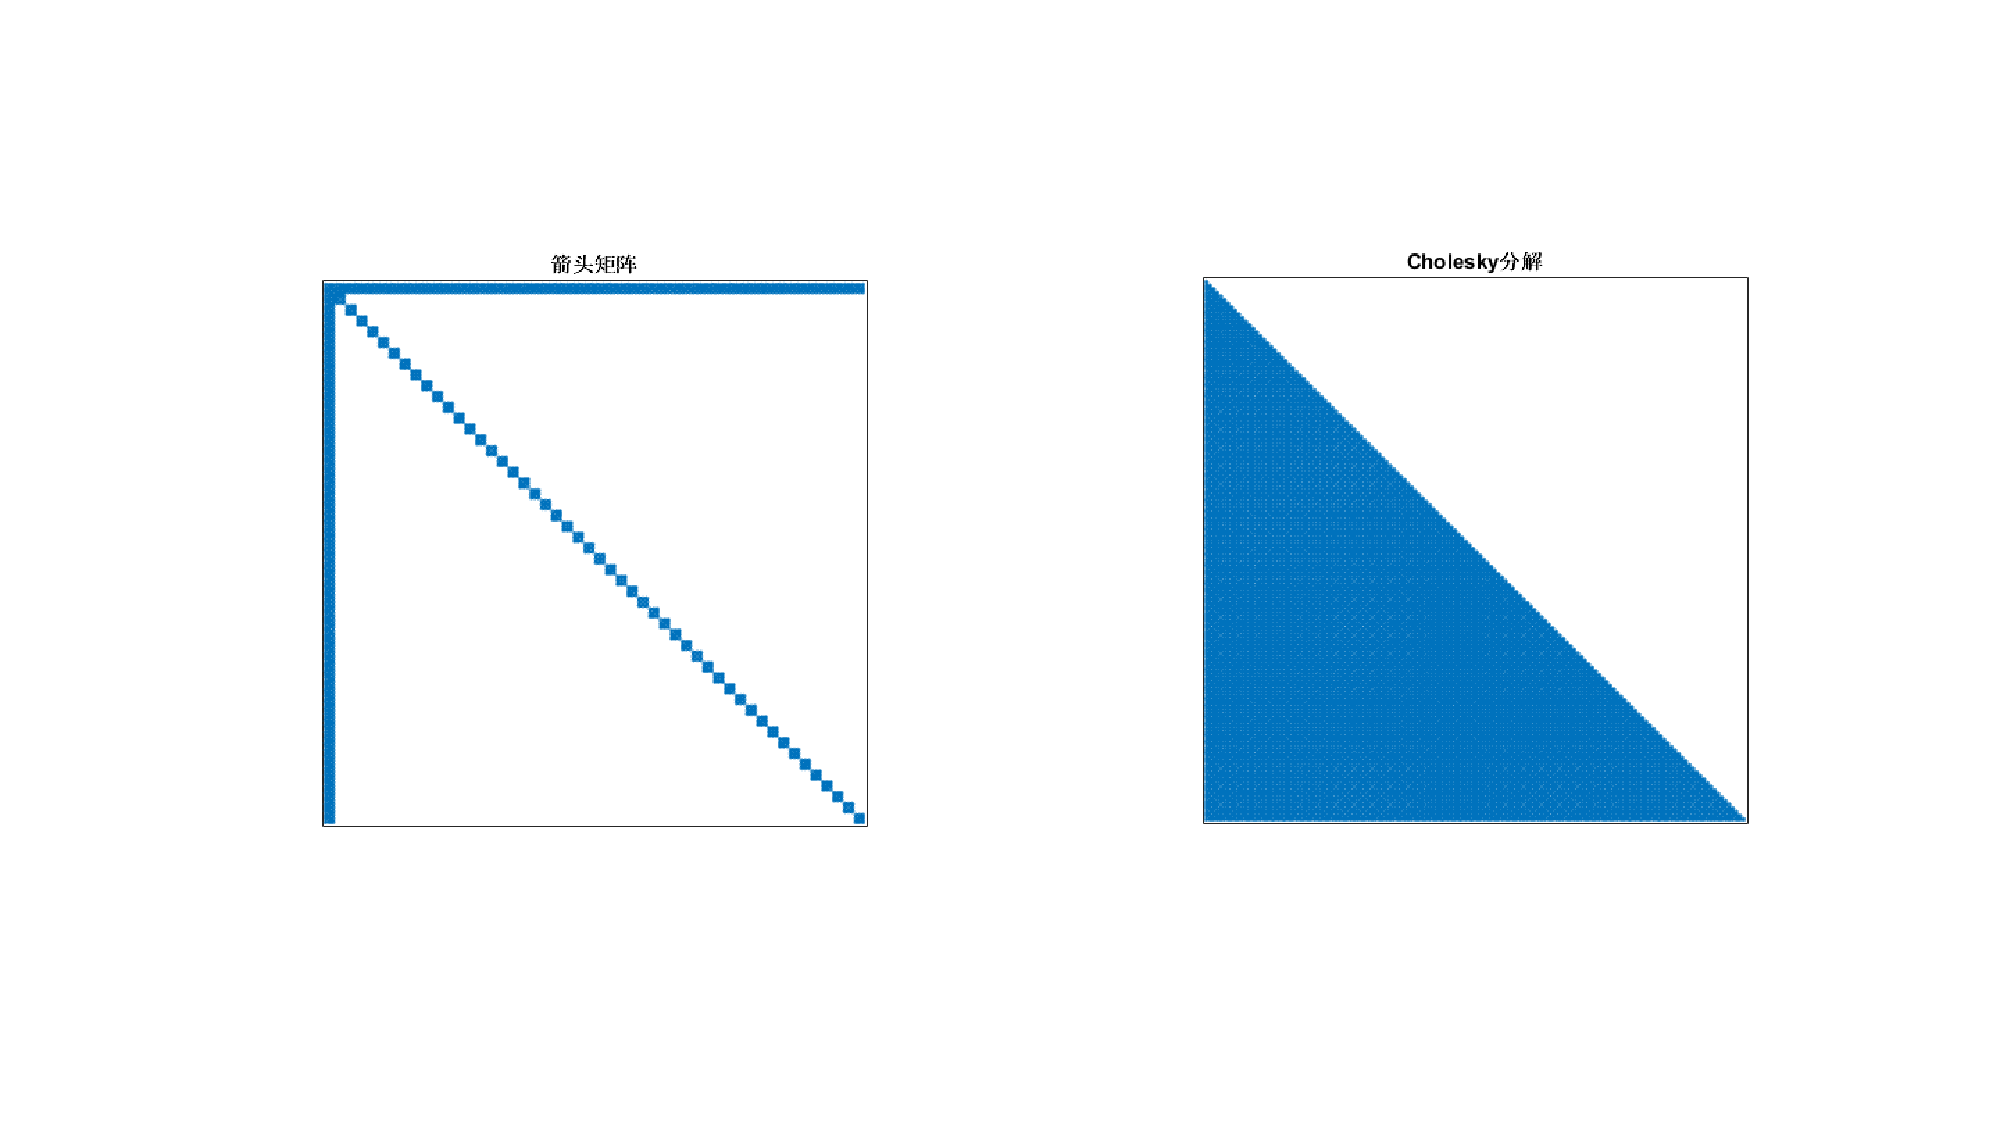
\includegraphics[width=0.8\textwidth]{backend1/arrowMatrix.pdf}
%	\caption{箭头矩阵(左)和其对应的Cholesky分解矩阵(右),Cholesky分解将原本稀疏的矩阵变成了稠密矩阵}
%	\label{fig:ArrowMatrix}
%\end{figure}
%
%由于我们对矩阵进行Cholesky分解的目的是为了求解线性方程组$\bm{Sx=p}$,我们可以改变向量$\bm{x}$当中的元素顺序,这种改变也只是需要对$\bm{S}$当中的非零成员出现的位置,不需要对$\bm{S}$进行重新计算。比如针对\autoref{fig:ArrowMatrix}的箭头矩阵所对应的线性系统$\bm{Sx=p}$来说,我们将整个$\bm{x}$当中所有变量的顺序颠倒,那么其对应的$\bm{S}$矩阵以及它的Cholesky分解就会出现\autoref{fig:ArrowMatrixPermute}这样的情况,Cholesky分解后依然是个稀疏矩阵,甚至连稀疏的图案都和原矩阵一模一样。
%
%\begin{figure}[!htp]
%	\centering
%	\includegraphics[width=0.8\textwidth]{backend1/arrowMatrixPermute.pdf}
%	\caption{调换顺序箭头矩阵(左)和其对应的Cholesky分解矩阵(右),Cholesky分解后依然是稀疏矩阵,并且和原矩阵具有一模一样的稀疏形式。}
%	\label{fig:ArrowMatrixPermute}
%\end{figure}
%
%显而易见,这样被排序后不但丝毫不影响线性方程组的求解,甚至我们在做后面的正向或者逆向代入法的时候,由于分解保持了稀疏性可以节约大量的乘法和加法运算从而提高了计算效率。同时,更具有吸引力的是,我们依然可以用原来稀疏矩阵的数据结构保存这个Cholesky分解后的矩阵,我们也不需要开辟新的存储空间,直接在原有的数据结构上不断计算和覆盖即可。如果是排序前\eqref{fig:ArrowMatrix}那类情况就太糟糕了,我们不仅需要更多的内存空间来保存这个矩阵,同时也需要更换这个矩阵的数据结构(用Hash表这类对付稀疏矩阵的数据结构来保存稠密矩阵将是个复杂低效的方法)。由此在对稀疏矩阵进行线性方程组求解之前,为了更加高效我们最好先使用\textbf{排序}(ordering)这类操作来尽可能避免过多的填充现象。
%
%至于这类减少填充的排序的算法,由于种类及其繁多,读者可以参考\cite{agarwal2012variable}。其中非常具有影响力的是EMD算法(Exact Minimum Degree),该算法针对矩阵对应的图不断地选取具有\textbf{最小度}(Degree)的节点而得到该矩阵对应的顺序。但值得说明的是,这种排序算法都是\textbf{NP难}问题(NP-complete,即在多项式时间内无法保证解决的问题)。正是因为如此,这里我也需要提醒读者,并不是所有排序都能使得整个线性系统变得更加快速。因此,为了真正保证有加速的作用,建议读者还是运行比较一下两者的运行时间从而进行选择。
%
%\subsection{QR分解求解Bundle Adjustment }
%Bundle Adjustment的解决方法也不止我们上面详细介绍的这一种,例如我们接下来将简单地介绍一类方法可以避免解算$\bm{H}$矩阵,直接通过QR分解来求解最小二乘方程\eqref{eq:BAleastsquare}。
%
%QR分解是将矩阵分解为单位正交矩阵$\bm{Q}$和上三角矩阵$\bm{R}$的操作,即$\bm{J=QR}$。QR分解的方法也有很多,例如给定旋转(Given Rotation),Householder 变换,Gram-Schmidt正交化等,这里不一一介绍,具体可以参考\cite{golub2012matrix}。QR分解当中一个非常重要的定理,就是当$\bm{J}$的维度是$m \times n, (m \ge n)$,且列满秩矩阵的时候,矩阵$\bm{J}$的QR分解为如下形式:
%
%\begin{displaymath}
%\bm{J=QR} = \left( {{{\bm{Q}}_1},{{\bm{Q}}_2}} \right)\left( {\begin{array}{*{20}{c}}
%		{{\bm{R}_1}}\\
%		 \bm{0}
%		\end{array}} \right) = \bm{Q}_1 \bm{R}_1
%\end{displaymath}
%
%此时$\bm{J=Q_1 R_1}$是该分解的\textbf{紧凑形式}(thin QR decomposition),其中 $\bm{Q_1} \in \bm{\mathbb{R}^{m \times n}}$,由一系列单位正交的列向量组成(即$\bm{Q_1^TQ_1 = I_n}$);同时$\bm{R_1}$是维度为$n \times n$的上三角矩阵,而且对角线元素均大于0。
%
%由于$\bm{Q}$是单位正交矩阵,我们有${\left\| \bm{Q^Ty} \right\|_2} = {\left\| \bm{y} \right\|_2}$,所以我们不难推出:
%
%\begin{align*}
%\left\| \bm{Jx + f} \right\|^2 &= 
%\left\| (\bm{Q_1},\bm{Q_2})(\begin{array}{*{20}{c}}
%		\bm{R}_1\\
%		\bm{0}
%		\end{array})\bm{x} + \bm{f} \right\|^2 \\ &= 
%\left\| \left( \begin{array}{*{20}{c}}
%			\bm{Q}_1^T\\
%			\bm{Q}_2^T
%			\end{array} \right)(\bm{Q_1},\bm{Q_2})(\begin{array}{*{20}{c}}
%		\bm{R}_1\\
%		\bm{0}
%		\end{array})\bm{x} + \left( \begin{array}{*{20}{c}}
%			\bm{Q}_1\\
%			\bm{Q}_2
%			\end{array} \right)\bm{f} \right\|^2 \\ &= 
%\left\| \bm{R_1 x} + \bm{Q}_1^T\bm{f} \right\|^2 + \left\| \bm{Q}_2^T\bm{f} \right\|^2
%\end{align*}
%
%这样,我们不难看出,由于$\bm{R_1}$是上三角矩阵,该最小二乘的最优解就是用前面提到的逆向代入法求解方程组:
%
%\begin{displaymath}
%\bm{R_1 x} = -\bm{Q_1^T f}
%\end{displaymath}
%
%该方法也同样需要讲究使用前面的排序手段来保持矩阵$\bm{R}_1$的稀疏性,但由于该分解方法远远没有Schur消元后进行Cholesky分解的方法快速,现实中很少采纳。但值得一提的是,QR分解却是比Cholesky分解数值上更加稳定的方法。
%
%线性系统的稳定性是实战中不可忽略的分析部分,因为由于处理器精度的限制(例如双精度浮点数只有16位有效数字,则精度的数量级是$10^{-16}$),有的低端处理器又只能让你使用单精度浮点数,因此任何情况下我们对矩阵的计算都存在截断误差。这种截断误差对矩阵的影响,可以说是对矩阵的一种\textbf{扰动},我们并不希望这类扰动对最后的求解结果带来太大影响。具体的分析需要用到矩阵的\textbf{条件数}(Condition number),这又是一些复杂的数学内容,我推荐希望深入的读者参考书籍\cite{golub2012matrix}。但需要我们记住的是,相比前面提到的Cholesky分解而言,QR分解是个速度慢但是数值上更稳定的选择。

\subsection{鲁棒核函数}
在前面的BA问题中,我们最小化误差项的二范数平方和作为目标函数。这种做法虽然很直观,但存在一个严重的问题:如果出于误匹配等原因,某个误差项给的数据是错误的,会发生什么呢?我们把一条原本不应该加到图中的边给加进去了,然而优化算法并不能辨别出这是个错误数据,它会把所有的数据都当作误差来处理。这时,算法会看到一条误差很大的边,它的梯度也很大,意味着调整与它相关的变量会使目标函数下降更多。所以,算法将试图调整这条边所连接的节点的估计值,使它们顺应这条边的无理要求。由于这条边的误差真的很大,往往会抹平了其他正确边的影响,使优化算法专注于调整一个错误的值。这显然不是我们希望看到的。

出现这种问题的原因是,当误差很大时,二范数增长得太快。于是就有了核函数的存在。核函数保证每条边的误差不会大得没边而掩盖掉其他的边。具体的方式是,把原先误差的二范数度量替换成一个增长没有那么快的函数,同时保证自己的光滑性质(不然无法求导!)。因为它们使得整个优化结果更为稳健,所以又叫它们鲁棒核函数(Robust Kernel)。

鲁棒核函数有许多种,例如最常用的Huber核:
\begin{equation}
H\left( e \right) = 
\left\{ 
\begin{array}{ll}
\frac{1}{2}{e^2} &\quad \text{当} |e| \leqslant \delta, \\
\delta \left( {\left| e \right| - \frac{1}{2}\delta } \right) &\quad \text{其他}
\end{array} \right.
\end{equation}

我们看到,当误差$e$大于某个阈值$\delta$后,函数增长由二次形式变成了一次形式,相当于限制了梯度的最大值。同时,Huber核函数又是光滑的,可以很方便地求导。\autoref{fig:huber}~显示了Huber核函数与二次函数的对比,可见在误差较大时Huber核函数增长明显低于二次函数。

\begin{figure}[!htp]
	\centering
	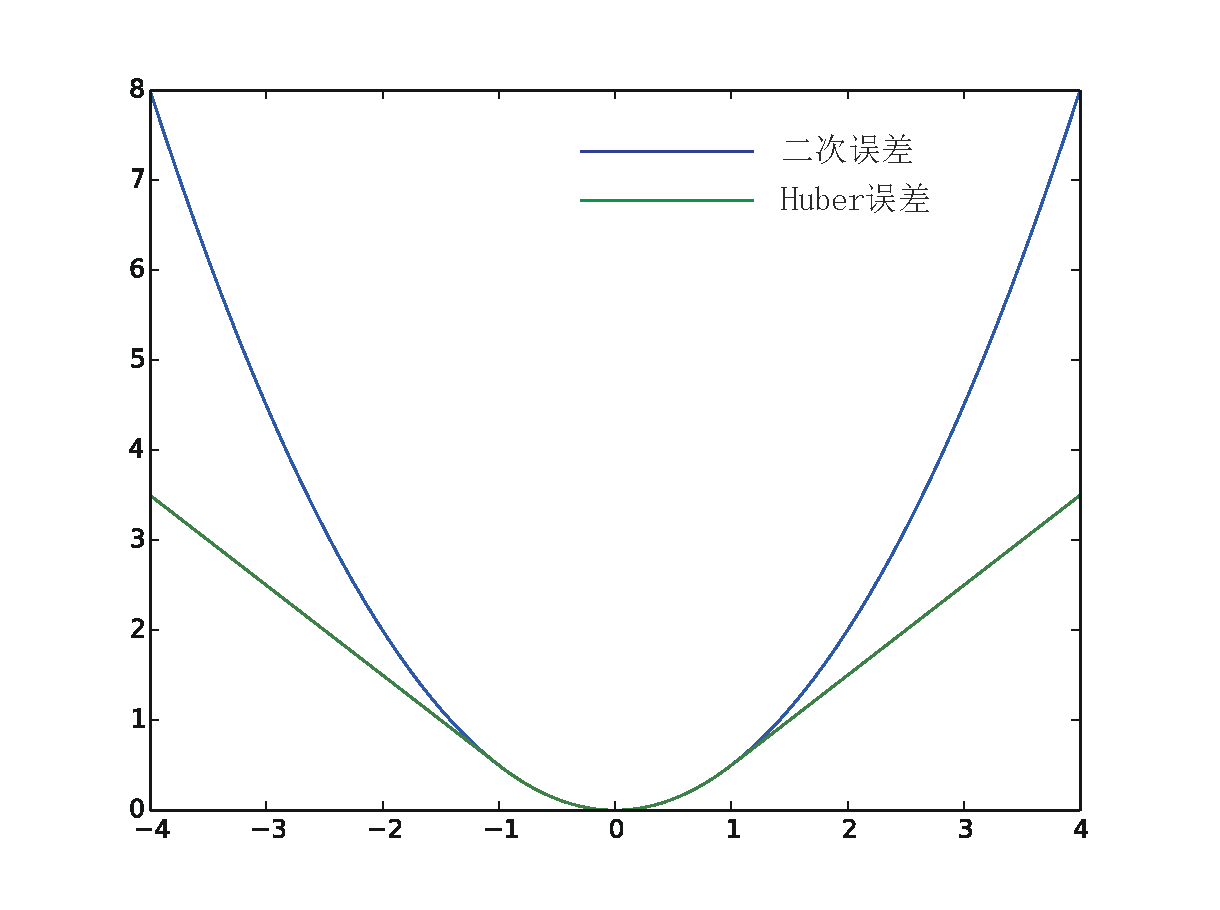
\includegraphics[width=0.5\textwidth]{backend1/huberloss}
	\caption{Huber核函数。}
	\label{fig:huber}
\end{figure}

除了Huber核之外,还有Cauchy核、Tukey核,等等,读者可以看看g2o和Ceres都提供了哪些核函数。

\subsection{小结}
%由于本书是围绕SLAM来谈的书籍,所以在这里只打算谈及SLAM种最常用的技术。Bundle Adjustment往往是个大型的稀疏问题,尽管我们可以用QR分解来求,但是由于$\bm{J}$往往太大,QR分解速度很慢,因此实际当中QR分解方法通常用来求解小维度并且实时性要求不太高的问题。

%Choleksy分解是Bundle Adjustment 常用的手段之一,但却不是唯一的。如果是非常大规模的三维重建(例如从社交网络的图片采集进行三维重建),这个数据量远远比SLAM里面的一个局部Bundle Adjustment要大很多,以至于进行Schur消元法$\bm{S} = \bm{B} - \bm{E}\bm{C}^{-1}\bm{E}^T$都需要大量计算,并且在Cholesky分解之后得到稠密的三角矩阵 依然还是会留下一个非常庞大的矩阵,上述介绍的排序然后再求解的方法并不管用,往往使用PCG(Preconditioned Conjugate Gradients)\cite{agarwal2010bundle}来解决。

%但不管是采用Cholesky方法还是PCG,排序方法是很多,但幸运的是,SLAM里面我们不太需要操作矩阵怎么排序,因为许多优秀的稀疏矩阵库已经实现了。
本节我们重点介绍了BA中的稀疏性问题。不过,实践当中,有许多软件库为我们提供了细节操作,而我们需要做的主要是构造Bundle Adjustment问题,设置Schur消元,然后调用稠密或者稀疏矩阵求解器对变量进行优化即可。如果读者希望更深入地了解BA,可以在阅读完本节的基础上,进一步参考文献\cite{Triggs2000}学习。

下面的两节,我们将使用g2o和Ceres两个库来做Bundle Adjustment。为了体现出它们的区别,我们会让这个程序共用很多代码。共用的代码主要在common文件夹下,其他的文件则不同。我们将使用公开的数据库\cite{bundleadjustmentinlarge}当中的文件来进行编程练习。
\clearpage

\section{实践:g2o}
\subsection{BA数据集}

在本讲代码目录下的common文件夹是两个实验共有的数据集部分。它的布局如\autoref{fig:common}~所示。其中,flags文件夹下的两个文件定义了CommandArgs这个类,该类用来解析用户输入的参数,同时也对程序需要的参数提供默认值及文档说明。BundleParams这个类定义了Bundle Adjustment使用的所有参数,也调用了CommandArgs类型的变量。由于CommandArgs这个类的存在,我们可以直接在程序后面使用 -help 来查看程序所有参数的含义,使用方式可以参考该程序中BundleParams类型的写法。

\begin{figure}[!htp]
	\centering
	\includegraphics[width=0.45\textwidth]{backend1/common.jpg}
	\caption{common 文件夹目录结构。}
	\label{fig:common}
\end{figure}

tools是一些数学工具函数,读者可自行查看。我们的相机和路标参数与前面提到的代价函数,即式\eqref{eq:BAcostfunction}保持一致,不过在实验中我们要把相机内参也当作优化变量考虑。我们用$f,k_1,k_2$来表示焦距和畸变,3个参数表示平移,3个参数表示旋转(于是相机一共有9个未知量),路标也使用三维坐标来表示。projection.h是前面提到的投影计算流程\autoref{fig:calculationflow}~的代码实现。由于g2o和ceres都会用到这个投影模型,因此这个文件也将被两个工程所共享。

除此之外,BALProblem这个类将保存我们的Bundle Adjustment所需要的所有数据,其中就包括了相机和路标之间的关联,以及相机变量和路标变量的初始值,这些数据的原始信息都保存在data文件夹下的TXT文件当中。我们可以打开data/problem-16-22106-pre.txt查看文件信息:

\clearpage
\begin{lstlisting}
16 22106 83718
0 0     -3.859900e+02 3.871200e+02
1 0     -3.844000e+01 4.921200e+02
2 0     -6.679200e+02 1.231100e+02
7 0     -5.991800e+02 4.079300e+02
\end{lstlisting}

它的第一行记录了相机数量、路标数量和总的观测数量。从第二行起,分别记录第$i$个相机观测第$j$个路标所看到的像素坐标。这就构成了一个BA问题,亦可看成由纯观测方程组成的SLAM问题。除此之外,BALProblem也提供了将数据导出到PLY文件这样的功能,方便用户通过Meshlab软件查看点云的三维信息。

\subsection{g2o求解BA}
下面来考虑如何使用g2o求解这个BA问题。和以前一样,g2o使用图模型来描述问题的结构,所以我们要用节点来表示相机和路标,然后用边来表示它们之间的观测。我们仍然使用自定义的点和边,只需覆盖一些关键函数即可。针对相机和路标,我们可以定义如下继承,使用override关键字来表示对基类虚函数的覆盖:

\begin{lstlisting}[language=c++,caption=slambook/ch10/g2o_custombundle/g2o_bal_class.h]
#include "g2o/core/base_vertex.h"
#include "g2o/core/base_binary_edge.h"

#include <Eigen/Core>
#include "ceres/autodiff.h"

#include "tools/rotation.h"
#include "common/projection.h"

// 节点没什么好说的,直接把更新量看作向量求加法即可
class VertexCameraBAL : public g2o::BaseVertex<9,Eigen::VectorXd>
{
public:
	EIGEN_MAKE_ALIGNED_OPERATOR_NEW;
	VertexCameraBAL(){}
	virtual bool read(std::istream& is) {return false;}       
	virtual bool write ( std::ostream& os ) const {return false;}
	virtual void setToOriginImpl(){}

	virtual void oplusImpl(const double* update) override {
		Eigen::VectorXd::ConstMapType v(update, VertexCameraBAL::Dimension);
		_estimate += v;
	}	
};

class VertexPointBAL : public g2o::BaseVertex<3, Eigen::Vector3d>
{
public:
	EIGEN_MAKE_ALIGNED_OPERATOR_NEW;
	VertexPointBAL(){}
	virtual bool read( std::istream& is) {return false;}
	virtual bool write(std::ostream& os) const {return false;}
	virtual void setToOriginImpl() {}
	virtual void oplusImpl(const double* update) override {
		Eigen::Vector3d::ConstMapType v(update);
		_estimate += v;
	}
};
\end{lstlisting}

定义了节点以后,还需要定义边来表示节点之间的联系。每一条边都对应了一个代价函数\eqref{eq:BAcostfunction},同时为了避免复杂的求导运算,我们借助Ceres库当中的Autodiff(即自动求导)功能。该功能需要类型将需要求导的公式实现在括号运算符operator()里,代码如下:
\enlargethispage{4pt}
\begin{lstlisting}[language=c++,caption=slambook/ch10/g2o_custombundle/g2o_bal_class.h]
class EdgeObservationBAL : public g2o::BaseBinaryEdge<2, Eigen::Vector2d,VertexCameraBAL, VertexPointBAL>{
public:
	EIGEN_MAKE_ALIGNED_OPERATOR_NEW;
	EdgeObservationBAL(){}

	virtual bool read(std::istream& /*is*/){ return false;}

	virtual bool write(std::ostream& /*os*/)const { return false;}

	virtual void computeError() override   // 覆盖基类函数,使用operator()计算代价函数
	{
		const VertexCameraBAL* cam = static_cast<const VertexCameraBAL*>(vertex(0));
		const VertexPointBAL* point = static_cast<const VertexPointBAL*>(vertex(1));

		(*this)(cam->estimate().data(), point->estimate().data(), _error.data());
	}
	
	// 为了使用 Ceres 求导功能而定义的函数,让本类成为拟函数类
	template<typename T>
	bool operator()( const T* camera, const T* point, T* residuals  )const 
	{
		T predictions[2];
		CamProjectionWithDistortion(camera, point, predictions);
		residuals[0] = predictions[0] - T(measurement()(0));
		residuals[1] = predictions[1] - T(measurement()(1));
		return true;
	}

	virtual void linearizeOplus() override
	{
		const VertexCameraBAL* cam = static_cast<const VertexCameraBAL*>(vertex(0));
		const VertexPointBAL* point = static_cast<const VertexPointBAL*>(vertex(1));
		typedef ceres::internal::AutoDiff<EdgeObservationBAL, double, VertexCameraBAL::Dimension, VertexPointBAL::Dimension> BalAutoDiff;

		Eigen::Matrix<double, Dimension, VertexCameraBAL::Dimension, Eigen::RowMajor> dError_dCamera;
		Eigen::Matrix<double, Dimension, VertexPointBAL::Dimension, Eigen::RowMajor> dError_dPoint;
		double *parameters[] = { const_cast<double*>(cam->estimate().data()), const_cast<double*>(point->estimate().data()) };
		double *jacobians[] = { dError_dCamera.data(), dError_dPoint.data() };
		double value[Dimension];
		// Ceres 中的自动求导函数用法,需要提供 operator() 函数成员
		bool diffState = BalAutoDiff::Differentiate(*this, parameters, Dimension, value, jacobians);  

		// copy over the Jacobians (convert row-major -> column-major)
		if (diffState) {
			_jacobianOplusXi = dError_dCamera;
			_jacobianOplusXj = dError_dPoint;
		} else {
			assert(0 && "Error while differentiating");
			_jacobianOplusXi.setZero();
			_jacobianOplusXi.setZero();
		}
	}
};
\end{lstlisting}

以上定义了本问题中使用的节点和边。下面需要根据BALProblem类当中的实际数据来生成一些节点和边,交给g2o进行优化。值得注意的是,为了充分利用BA中的稀疏性,需要在这里将路标中的setMarginalized属性设置为true。代码的主要片段如下:

\begin{lstlisting}[language=c++,caption=slambook/ch10/g2o_custombundle/g2o_bundle.cpp(片段)]
void BuildProblem(const BALProblem* bal_problem, g2o::SparseOptimizer* optimizer, const BundleParams& params)
{
	const int num_points = bal_problem->num_points();
	const int num_cameras = bal_problem->num_cameras();
	const int camera_block_size = bal_problem->camera_block_size();
	const int point_block_size = bal_problem->point_block_size();

	// 添加相机和对应的初始值
	const double* raw_cameras = bal_problem->cameras();
	for(int i = 0; i < num_cameras; ++i)
	{
		ConstVectorRef temVecCamera(raw_cameras + camera_block_size * i,camera_block_size);
		VertexCameraBAL* pCamera = new VertexCameraBAL();
		pCamera->setEstimate(temVecCamera);   // 初始值
		pCamera->setId(i);           
		optimizer->addVertex(pCamera);
	}

	// Set point vertex with initial value in the dataset. 
	const double* raw_points = bal_problem->points();
	// const int point_block_size = bal_problem->point_block_size();
	for(int j = 0; j < num_points; ++j)
	{
		ConstVectorRef temVecPoint(raw_points + point_block_size * j, point_block_size);
		VertexPointBAL* pPoint = new VertexPointBAL();
		pPoint->setEstimate(temVecPoint);   // 点云的初始值
		pPoint->setId(j + num_cameras);     // 为了不和相机冲突,加上相机的 id

		// 设置该点在解方程时进行 Schur 消元
		pPoint->setMarginalized(true);
		optimizer->addVertex(pPoint);
	}

	// 为图添加边
	const int  num_observations = bal_problem->num_observations();
	const double* observations = bal_problem->observations();   

	for(int i = 0; i < num_observations; ++i)
	{	
		EdgeObservationBAL* bal_edge = new EdgeObservationBAL();
		const int camera_id = bal_problem->camera_index()[i]; // 使用前面的 id 获取相机
		const int point_id = bal_problem->point_index()[i] + num_cameras; // 使用前面的 id 获得点
		// Huber loss 函数(默认为不用设置)
		if(params.robustify)
		{
			g2o::RobustKernelHuber* rk = new g2o::RobustKernelHuber;
			rk->setDelta(1.0);
			bal_edge->setRobustKernel(rk);
		}
		// 设置边所对应的两个节点
		bal_edge->setVertex(0,dynamic_cast<VertexCameraBAL*>(optimizer->vertex(camera_id)));
		bal_edge->setVertex(1,dynamic_cast<VertexPointBAL*>(optimizer->vertex(point_id)));
		// 设置其协方差矩阵(在此处为单位矩阵)
		bal_edge->setInformation(Eigen::Matrix2d::Identity());
		// 设置边所对应的观测值
		bal_edge->setMeasurement(Eigen::Vector2d(observations[2*i+0],observations[2*i + 1]));
		
		optimizer->addEdge(bal_edge) ;
	}
}

\end{lstlisting}

\subsection{求解}
在使用g2o时,求解的设置无非这几种:1. 使用何种方法(列文伯格—马夸尔特方法、DogLeg等)来定义非线性优化的下降策略;2. 使用哪类线性求解器。注意到这里需要使用到稀疏性,所以必须选用稀疏的求解器。

\begin{lstlisting}[language=c++,caption=slambook/ch10/g2o_custombundle/g2o_bundle.cpp(片段)]
typedef g2o::BlockSolver<g2o::BlockSolverTraits<9,3> > BalBlockSolver;

void SetSolverOptionsFromFlags(BALProblem* bal_problem, const BundleParams& params, g2o::SparseOptimizer* optimizer)
{   
	BalBlockSolver* solver_ptr;
		
	g2o::LinearSolver<BalBlockSolver::PoseMatrixType>* linearSolver = 0;
	
	// 使用稠密计算方法
	if (params.linear_solver == "dense_schur" ) {
		linearSolver = new g2o::LinearSolverDense<BalBlockSolver::PoseMatrixType>();
	}
	// 使用稀疏计算方法
	else if (params.linear_solver == "sparse_schur") {
		linearSolver = new g2o::LinearSolverCholmod<BalBlockSolver::PoseMatrixType>();
		// 让 solver 对矩阵进行排序保持稀疏性
		dynamic_cast<g2o::LinearSolverCholmod<BalBlockSolver::PoseMatrixType>* >(linearSolver)->setBlockOrdering(true);  
	}
	
	solver_ptr = new BalBlockSolver(linearSolver);

	g2o::OptimizationAlgorithmWithHessian* solver;  
	if(params.trust_region_strategy == "levenberg_marquardt"){
		solver = new g2o::OptimizationAlgorithmLevenberg(solver_ptr);  // 使用列文伯格—马夸尔特下降法
	}
	else if(params.trust_region_strategy == "dogleg"){
		solver = new g2o::OptimizationAlgorithmDogleg(solver_ptr);  // 使用 DogLeg 下降法
	}
	else 
	{
		std::cout << "Please check your trust_region_strategy parameter again.."<< std::endl;
		exit(EXIT_FAILURE);
	}
	
	optimizer->setAlgorithm(solver);
}
	
\end{lstlisting}

现在问题基本上搭建好了。我们通过BuildProblem函数完成了对目标函数的构造,也通过SetSolverOptionsFromFlags函数使用用户的输入参数来设置优化求解。剩下要做的就是思考该如何求解这个问题了。有了g2o这样的优化库,求解基本上可以一步完成,这点跟前面介绍的g2o用法几乎是一样的:

\begin{lstlisting}[language=c++,caption=slambook/ch10/g2o_custombundle/g2o_bundle.cpp(片段)]
 optimizer.initializeOptimization();
 optimizer.setVerbose(true);
 optimizer.optimize(params.num_iterations);
\end{lstlisting}

\clearpage
使用Meshlab分别打开g2o执行文件夹下的initial.ply和final.ply两个文件,优化前后的效果如\autoref{fig:g2o-BA}~所示。

\begin{figure}[!htp]
	\centering
	\includegraphics[width=1.0\textwidth]{backend1/g2o-ba}
	\caption{g2o优化结果。左侧为优化前初始值,右侧为优化后的。}
	\label{fig:g2o-BA}
\end{figure}

由于g2o库本身公开API说明也少,我们通常只能通过网上的一些开源项目及其本身的源代码来了解它。这里需要提醒读者的是,g2o在做Bundle Adjustment的优化时必须将其所有点云全部Schur掉,否则会出错!其原因在于我们使用了g2o::LinearSolver\\<BalBlockSolver::PoseMatrixType>这个类型来指定linearsolver,其中模板参数当中的PoseMatrixType在程序中为相机姿态参数的维度,于是Bundle Adjustment当中Schur消元后解的线性方程组必须是只含有相机姿态变量\footnote{这种限制实在让人很懊恼。}。

Ceres库则没有g2o这样的限制。Ceres给了开发者很大的空间去操作自己的优化策略,它在Schur消元操作时完全不需要把所有点云都消元掉,用户可以自己编写函数选择消元哪些点云。接下来我们也会给出Ceres的BA示例。

\section{实践:Ceres}

现在我们再来看看换成Ceres实现同样的效果该如何做。如前面介绍的那样,Ceres是针对一般优化问题产生的库,因此它并没有像g2o那样提供一些Vertex或者Edge这类友好的接口。不过这也给Ceres带来了极大的灵活性。我们接下来可以看到,Ceres可以在原始数组上进行直接的优化操作,而g2o则通过复制的手段将数据通过Vertex或者Edge结构复制到optimizer里面。相比之下,Ceres对“优化”显得更贴近一些。

\subsection{Ceres求解BA}
g2o用Edge来保存每一个代价函数,而Ceres却是用Problem类型来构建最终的目标函数。与第6讲介绍的一致,我们使用AddResidualBlock来添加代价函数,最后组成整个目标函数。为了简化整个过程,我们首先定义代价函数类型,并且定义Create成员来使用Ceres当中的AutoDiff特性:

\begin{lstlisting}[language=c++,caption=slambook/ch10/ceres_custombundle/SnavelyReprojectionError.h]
class SnavelyReprojectionError
{
public:
	SnavelyReprojectionError(double observation_x, double observation_y):observed_x(observation_x),observed_y(observation_y){}

	template<typename T>
	bool operator()(const T* const camera, const T* const point, T* residuals)const
	{                  
		// camera[0,1,2] are the angle-axis rotation
		T predictions[2];
		CamProjectionWithDistortion(camera, point, predictions);
		residuals[0] = predictions[0] - T(observed_x);
		residuals[1] = predictions[1] - T(observed_y);

		return true;
	}

	static ceres::CostFunction* Create(const double observed_x, const double observed_y){
		return (new ceres::AutoDiffCostFunction<SnavelyReprojectionError,2,9,3>(
			new SnavelyReprojectionError(observed_x,observed_y)));
	}

private:
	double observed_x;
	double observed_y;
};
\end{lstlisting}

定义好之后,我们就可以使用SnavelyReprojectionError::Create函数来轻松地构建这个目标函数:

\begin{lstlisting}[language=c++,caption=slambook/ch10/ceres_custombundle/ceresBundle.cpp(片段)]
void BuildProblem(BALProblem* bal_problem, Problem* problem, const BundleParams& params)
{
	const int point_block_size = bal_problem->point_block_size();
	const int camera_block_size = bal_problem->camera_block_size();
	double* points = bal_problem->mutable_points();
	double* cameras = bal_problem->mutable_cameras();

	// Observations is 2 * num_observations long array observations
	// [u_1, u_2, ... u_n], where each u_i is two dimensional, the x 
	// and y position of the observation. 
	const double* observations = bal_problem->observations();

	for(int i = 0; i < bal_problem->num_observations(); ++i){
	CostFunction* cost_function;

	// Each Residual block takes a point and a camera as input 
	// and outputs a 2 dimensional Residual

	cost_function = SnavelyReprojectionError::Create(observations[2*i + 0], observations[2*i + 1]);

	// If enabled use Huber's loss function. 
	LossFunction* loss_function = params.robustify ? new HuberLoss(1.0) : NULL;

	// Each observation corresponds to a pair of a camera and a point 
	// which are identified by camera_index()[i] and point_index()[i]
	// respectively.
	double* camera = cameras + camera_block_size * bal_problem->camera_index()[i];
	double* point = points + point_block_size * bal_problem->point_index()[i];

	problem->AddResidualBlock(cost_function, loss_function, camera, point);
}
\end{lstlisting}

值得一提的是,为了使用Schur消元,Ceres采取的策略和g2o有很大的不同。Ceres采用额外的类型ParameterBlockOrdering来管理Schur消元顺序,并且使用AddElementToGroup来对变量进行编号从而定义消元顺序。例如下面设置点云变量为0,相机变量为1就可以让点云变量先进行消元(优先消元编号最小的变量):

\begin{lstlisting}[language=c++,caption=slambook/ch10/ceres_custombundle/ceresBundle.cpp]
void SetOrdering(BALProblem* bal_problem, ceres::Solver::Options* options, const BundleParams& params)
{
	const int num_points = bal_problem->num_points();
	const int point_block_size = bal_problem->point_block_size();
	double* points = bal_problem->mutable_points();

	const int num_cameras = bal_problem->num_cameras();
	const int camera_block_size = bal_problem->camera_block_size();
	double* cameras = bal_problem->mutable_cameras();

	if (params.ordering == "automatic")
		return;

	ceres::ParameterBlockOrdering* ordering = new ceres::ParameterBlockOrdering;

	// The points come before the cameras
	for(int i = 0; i < num_points; ++i)
		ordering->AddElementToGroup(points + point_block_size * i, 0);

	for(int i = 0; i < num_cameras; ++i)
		ordering->AddElementToGroup(cameras + camera_block_size * i, 1);

	options->linear_solver_ordering.reset(ordering);
}
\end{lstlisting}

\subsection{求解}

Ceres除了能够在原始数组上操作以外,另一大优势在于它的优化设置非常便捷。g2o的设置全靠变量类型来选择不同的下降策略,以及选择稠密或者稀疏的线性方程组解法,而Ceres全靠给Solver::Options的类型成员变量进行赋值来调整,这种方式比g2o快捷便利很多。Options类型几乎集成了Ceres的所有求解方法设置和管理,包括我们上面提到的Schur消元顺序(注意上面函数当中的最后一行)。

\begin{lstlisting}[language=c++,caption=slambook/ch10/ceres_custombundle/ceresBundle.cpp(片段)]
void SetSolverOptionsFromFlags(BALProblem* bal_problem,
const BundleParams& params, Solver::Options* options){
	
	options->max_num_iterations = params.num_iterations;
	options->minimizer_progress_to_stdout = true;
	options->num_threads = params.num_threads; // 用于计算的线程数目,可以加速雅可比矩阵的计算
	
	// 下降策略的选取
	CHECK(StringToTrustRegionStrategyType(params.trust_region_strategy,
	&options->trust_region_strategy_type)); 
	
	//  linear solver 的选取
	CHECK(ceres::StringToLinearSolverType(params.linear_solver, &options->linear_solver_type));
	CHECK(ceres::StringToSparseLinearAlgebraLibraryType(params.sparse_linear_algebra_library, &options->sparse_linear_algebra_library_type));
	CHECK(ceres::StringToDenseLinearAlgebraLibraryType(params.dense_linear_algebra_library, &options->dense_linear_algebra_library_type));
	
	// 变量排序的设置
	SetOrdering(bal_problem, options,params);
}

\end{lstlisting}

Ceres的求解也很简单。和前面提到的曲线拟合的例子一样,只需要简单地设置一下关于梯度和相邻两次迭代之间目标函数之差的相关阈值就可以。Solve函数负责Ceres的求解功能,只需要传给它对应的选项、目标函数即可。Summary类型用来负责函数求解每一次迭代的结果统计。

\begin{lstlisting}[language=c++,caption=slambook/ch10/ceres_custombundle/ceresBundle.cpp(片段)]
   options.gradient_tolerance = 1e-16;
   options.function_tolerance = 1e-16;
   Solver::Summary summary;
   Solve(options, &problem, &summary);
\end{lstlisting}

和g2o示例一样,该程序在运行后也可以在执行文件目录下找到final.ply文件和initial.ply,由于该程序和g2o程序采用一致的数据,因此initial.ply具有相同的图案。使用MeshLab软件打开final.ply可以看到如\autoref{fig:ceresfinal}~所示的结果,通过对比也可以发现优化结果和g2o完全一样。

\begin{figure}[!ht]
	\centering
	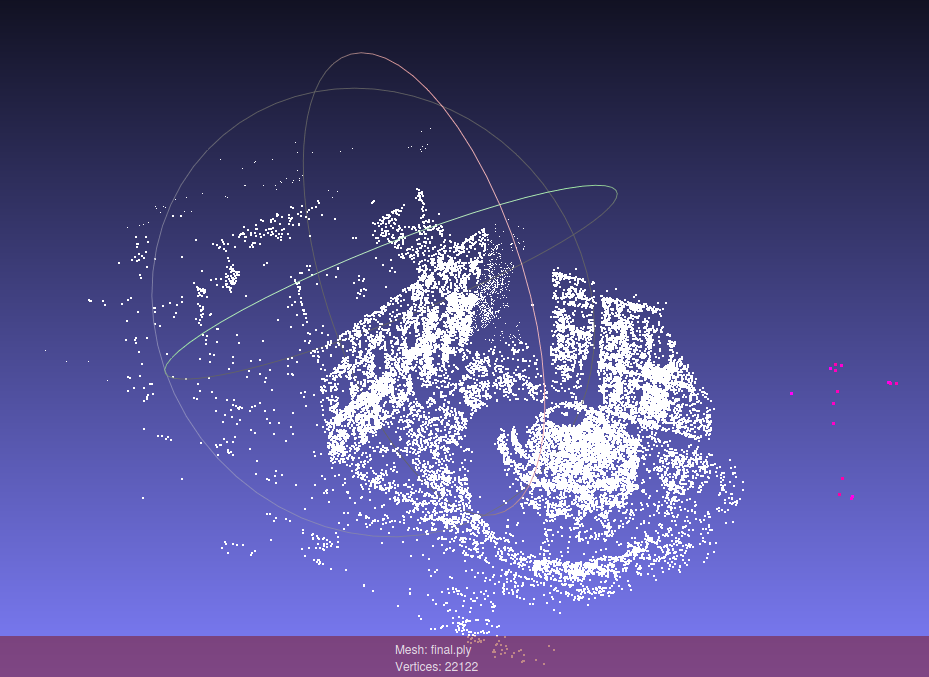
\includegraphics[width=0.72\textwidth]{backend1/final1.png}
	\caption{Ceres的优化结果。}
	\label{fig:ceresfinal}
\end{figure}

Ceres库公开的API说明详细,同时源代码可读性也高,推荐读者多多阅读Ceres源代码,并且自己尝试在Schur消元操作中只消去部分点云变量,或者夹杂着消去一些相机变量。这只需要操作ceres::ParameterBlockOrdering::AddElementToGroup函数,在对应变量地址上,用序号指定顺序即可。相比g2o这样公开文档太少的库,我们更加推荐读者更多地使用Ceres这样的库来做SLAM。

\section{小结}
本讲比较深入地探讨了状态估计问题与图优化的求解。我们看到在经典模型中SLAM可以看成状态估计问题。如果我们假设马尔可夫性,只考虑当前状态,则得到以EKF为代表的滤波器模型。如若不然,我们也可以选择考虑所有的运动和观测,它们构成一个最小二乘问题。在只有观测方程的情况下,这个问题称为BA,并可利用非线性优化方法求解。我们仔细讨论了求解过程中的稀疏性问题,指出了该问题与图优化之间的联系。最后,我们演示了如何使用g2o和Ceres库求解同一个优化问题,让读者对BA有一个直观的认识。

\section*{习题}
\begin{enumerate}
	\item 证明式\eqref{eq:kalman-K-another}成立。提示:你可能会用到SMW(Sherman-Morrison-Woodbury)公式,参考文献\cite{Sherman1950, Barfoot2016}。
	\item 
	对比g2o和Ceres的优化后目标函数的数值。指出为什么两者在Meshlab中效果一样但数值却不同。
	\item 
	对Ceres当中的部分点云进行Schur消元,看看结果会有什么区别。
	\item 证明$\bm{S}$矩阵为半正定矩阵。
	\item 阅读文献\cite{Kummerle2011},看看g2o对核函数是如何处理的。与Ceres中的Loss function有何联系?
	\item[\optional] 在两个示例中,我们优化了相机位姿、以$f, k_1, k_2$为参数的相机内参及路标点。请考虑使用第5讲介绍的完整的相机模型进行优化,即,至少考虑$f_x, f_y, p_1, p_2,$ $k_1, k_2$这些量。修改现在的Ceres和g2o程序以完成实验。
\end{enumerate}
